\documentclass{article}
\usepackage[utf8]{inputenc}
\usepackage{enumerate}

% image-related packages
\usepackage{wrapfig}
\usepackage{subcaption}
\usepackage{float, graphicx}
\graphicspath{{./Image/}}
\usepackage[export]{adjustbox}
%----------------------------------



\title{BCL2 Family Expression According to The Subgroup of DLBCL}
\author{Jin Roh}
\date{\today}

\begin{document}

\maketitle

\section*{Topic 1 Descriptive analysis}

\begin{enumerate}
    \item Heatmap of BCL2 family expression (rescaled)
    
    \begin{figure}[H]
        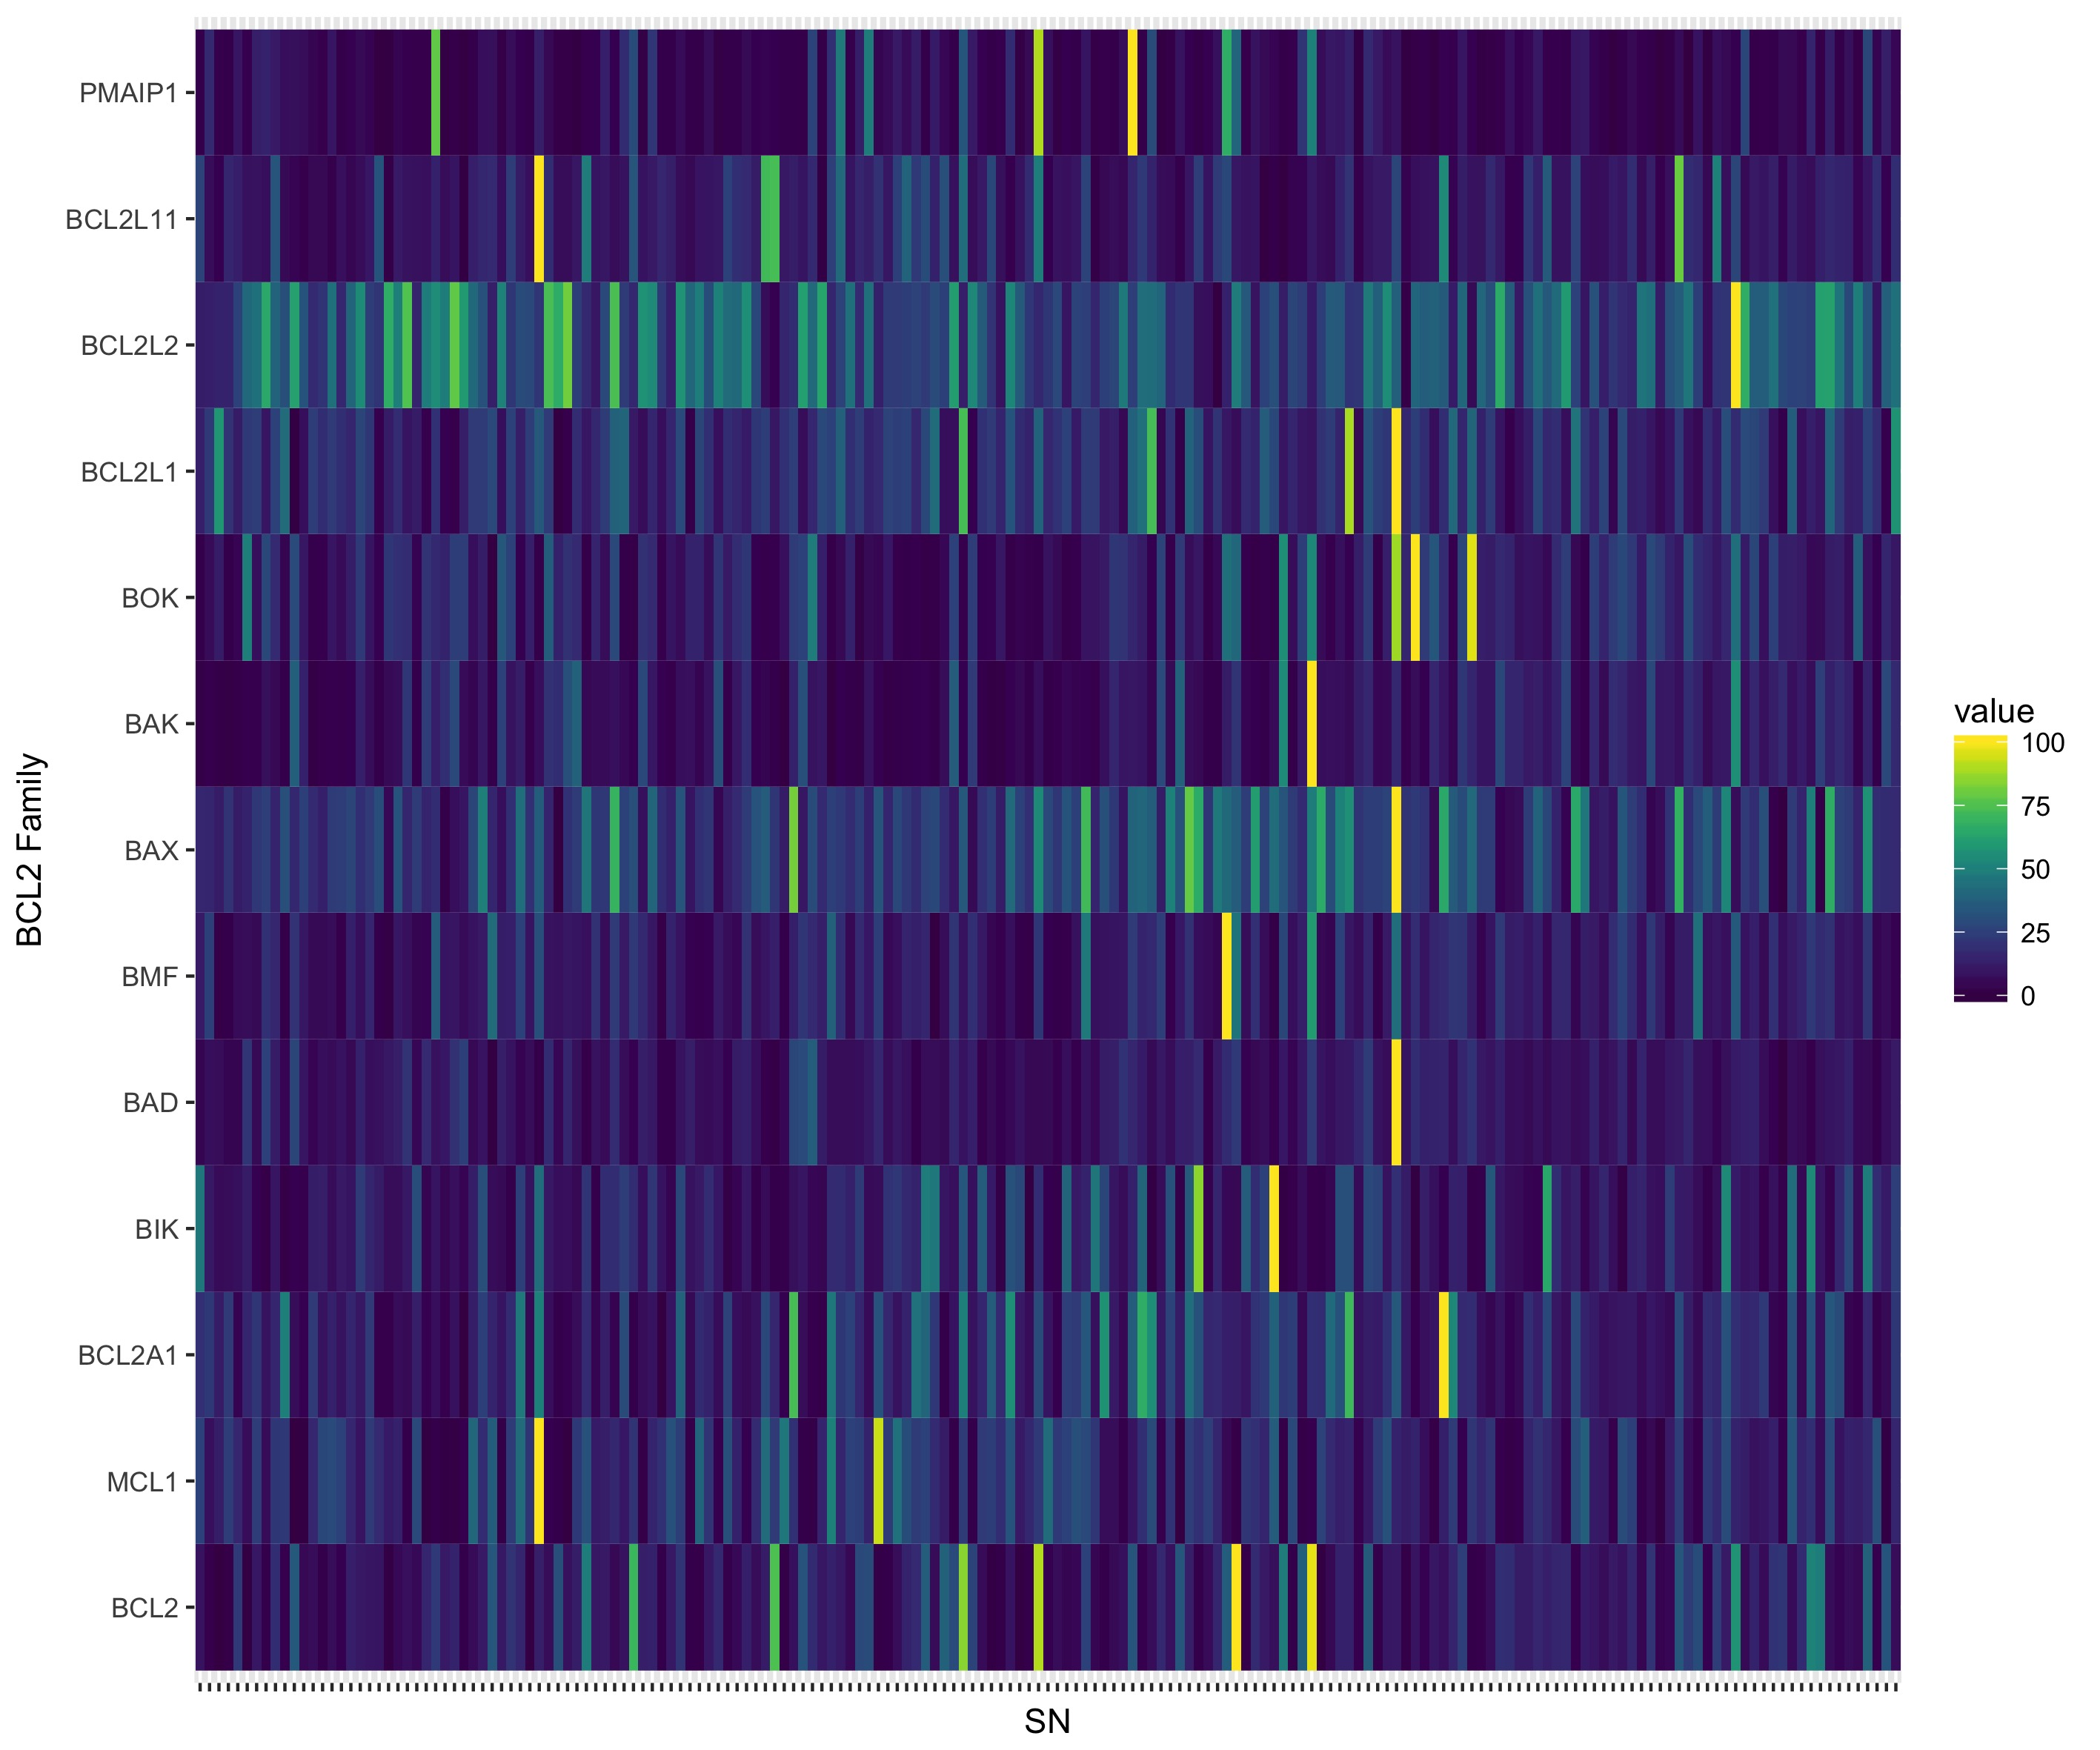
\includegraphics[width = 0.8\textwidth, center]{Image/BCL2_Heatmap.jpg}
    \end{figure}
    
\end{enumerate}

\section*{Topic 2 Dimention Reduction and Clustering}

\begin{enumerate}
    \item t-SNE
    
    \begin{figure}[H]
    
        \begin{subfigure}{0.5\textwidth}
        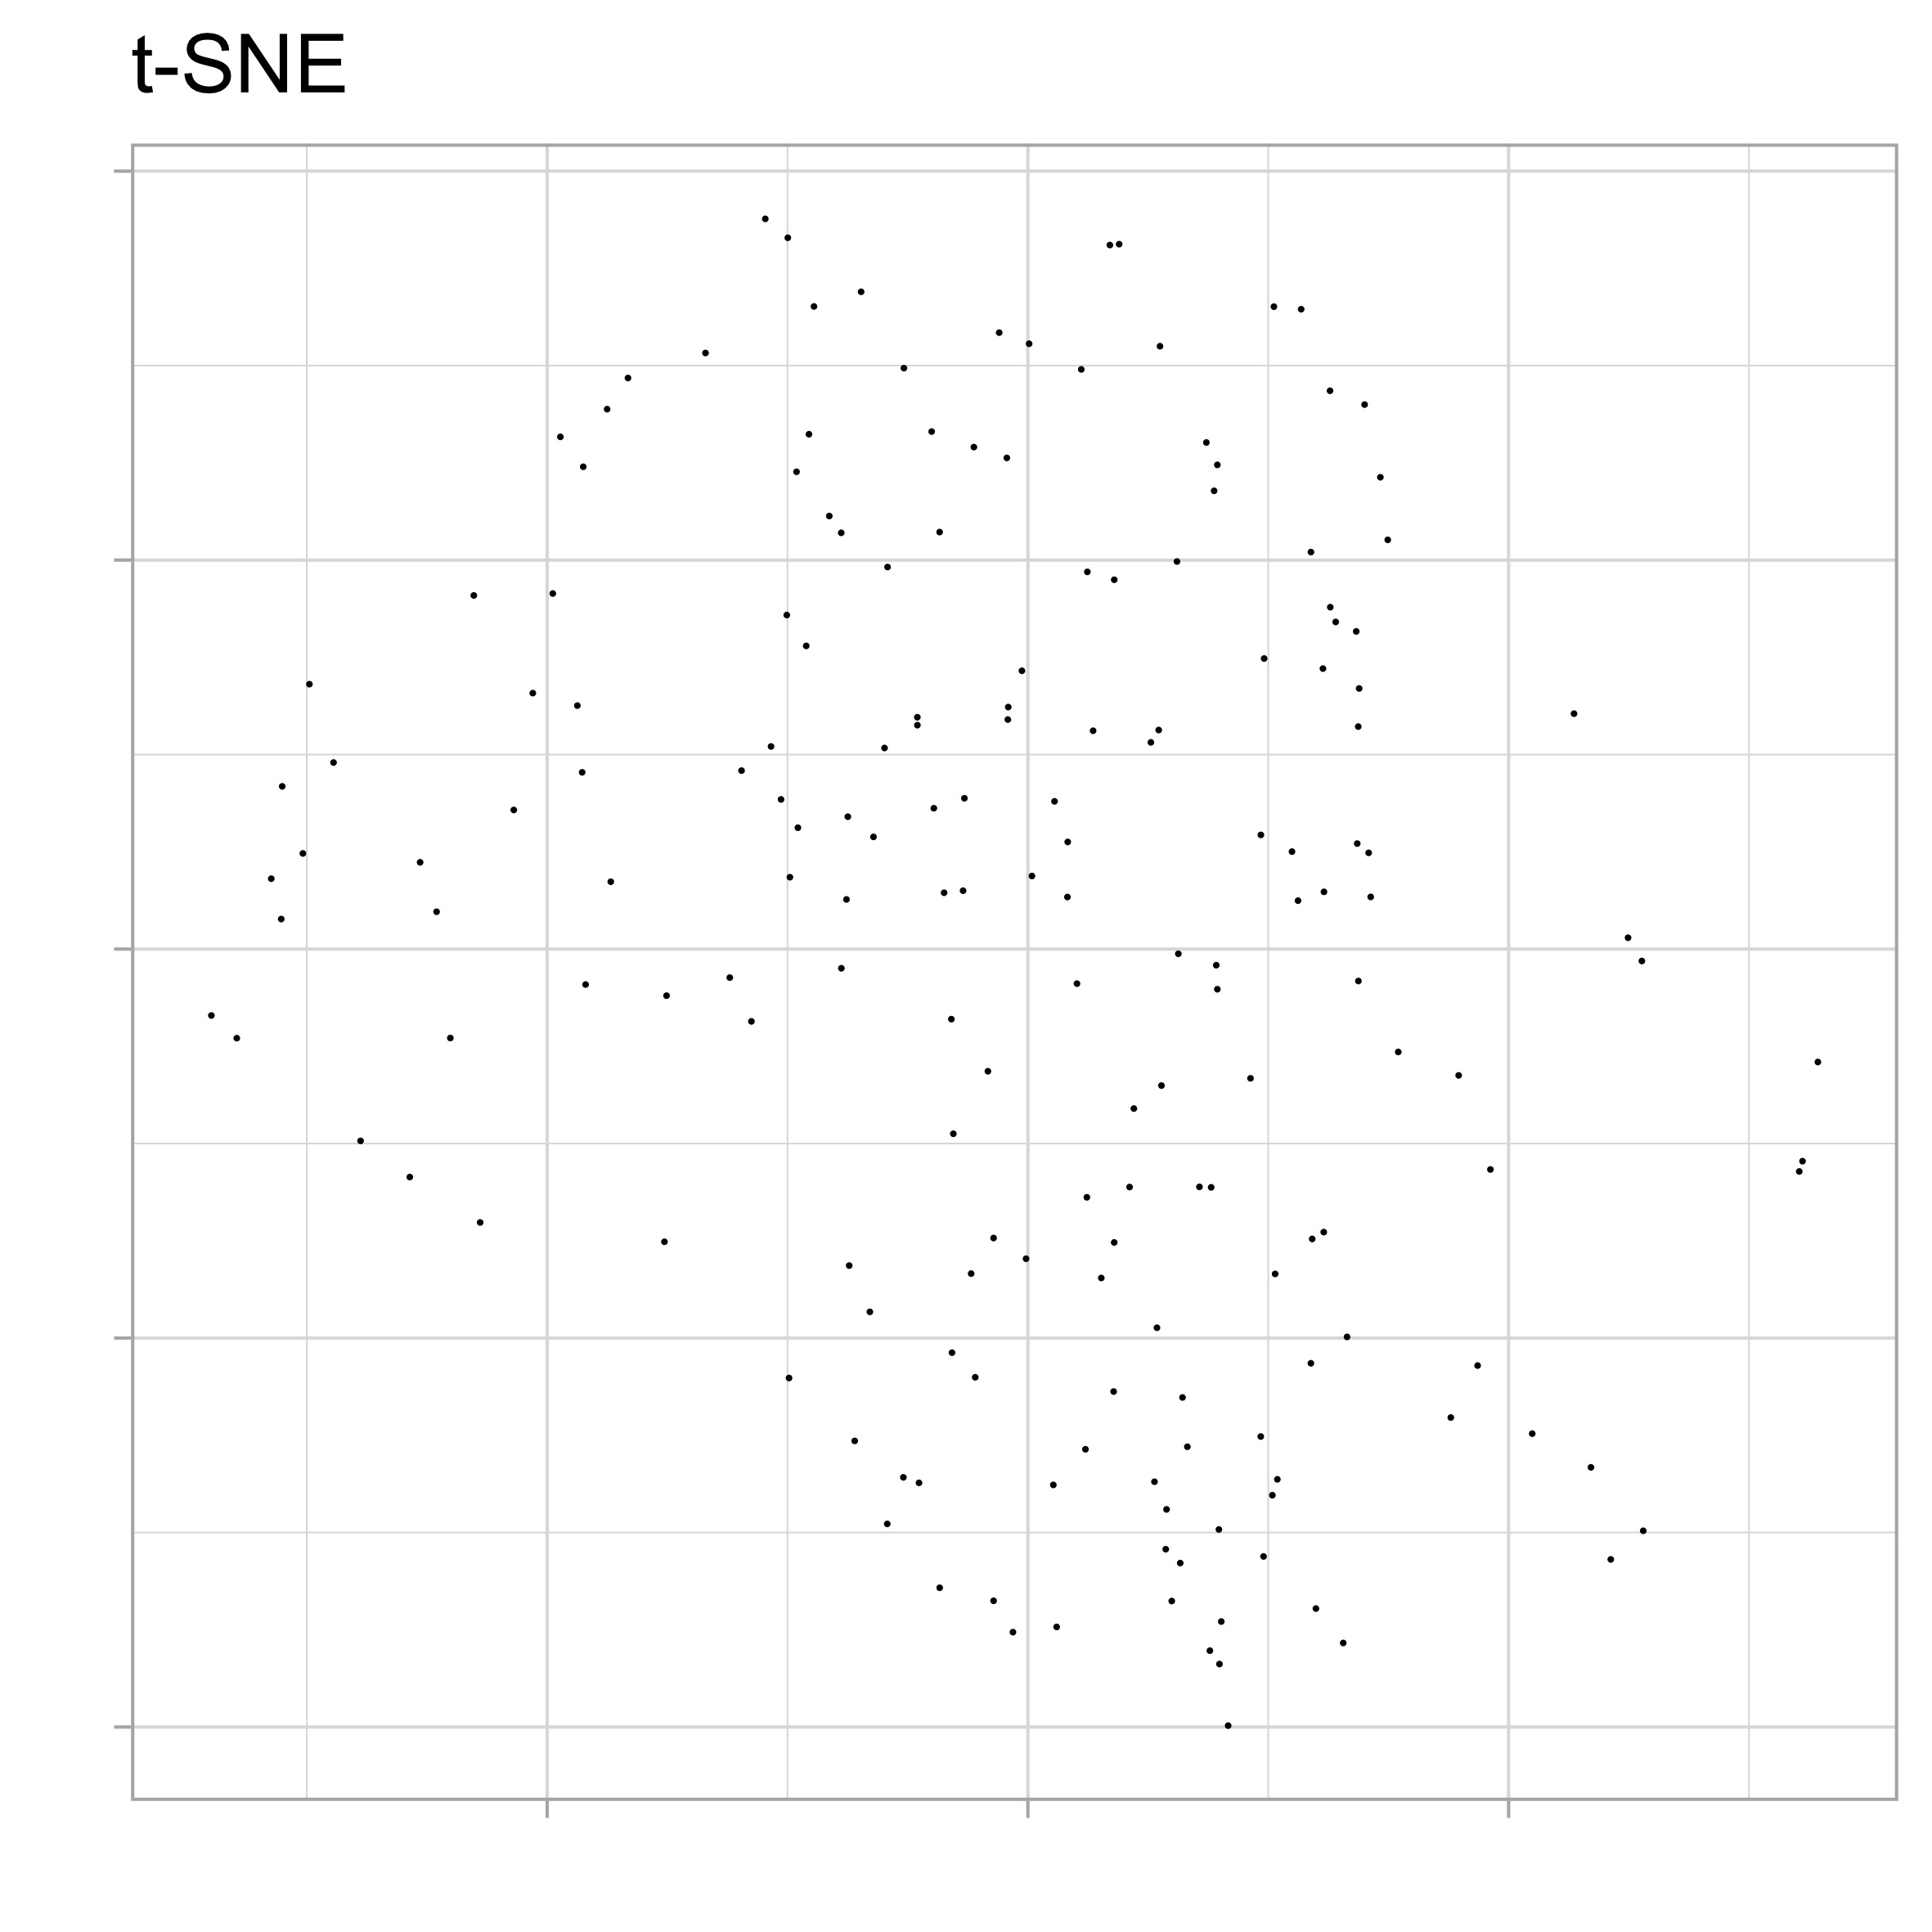
\includegraphics[width = 0.9\linewidth, height = 5cm]{Image/t-SNE.jpg}
        \caption{t-SNE}
        \end{subfigure}
        \begin{subfigure}{0.5\textwidth}
        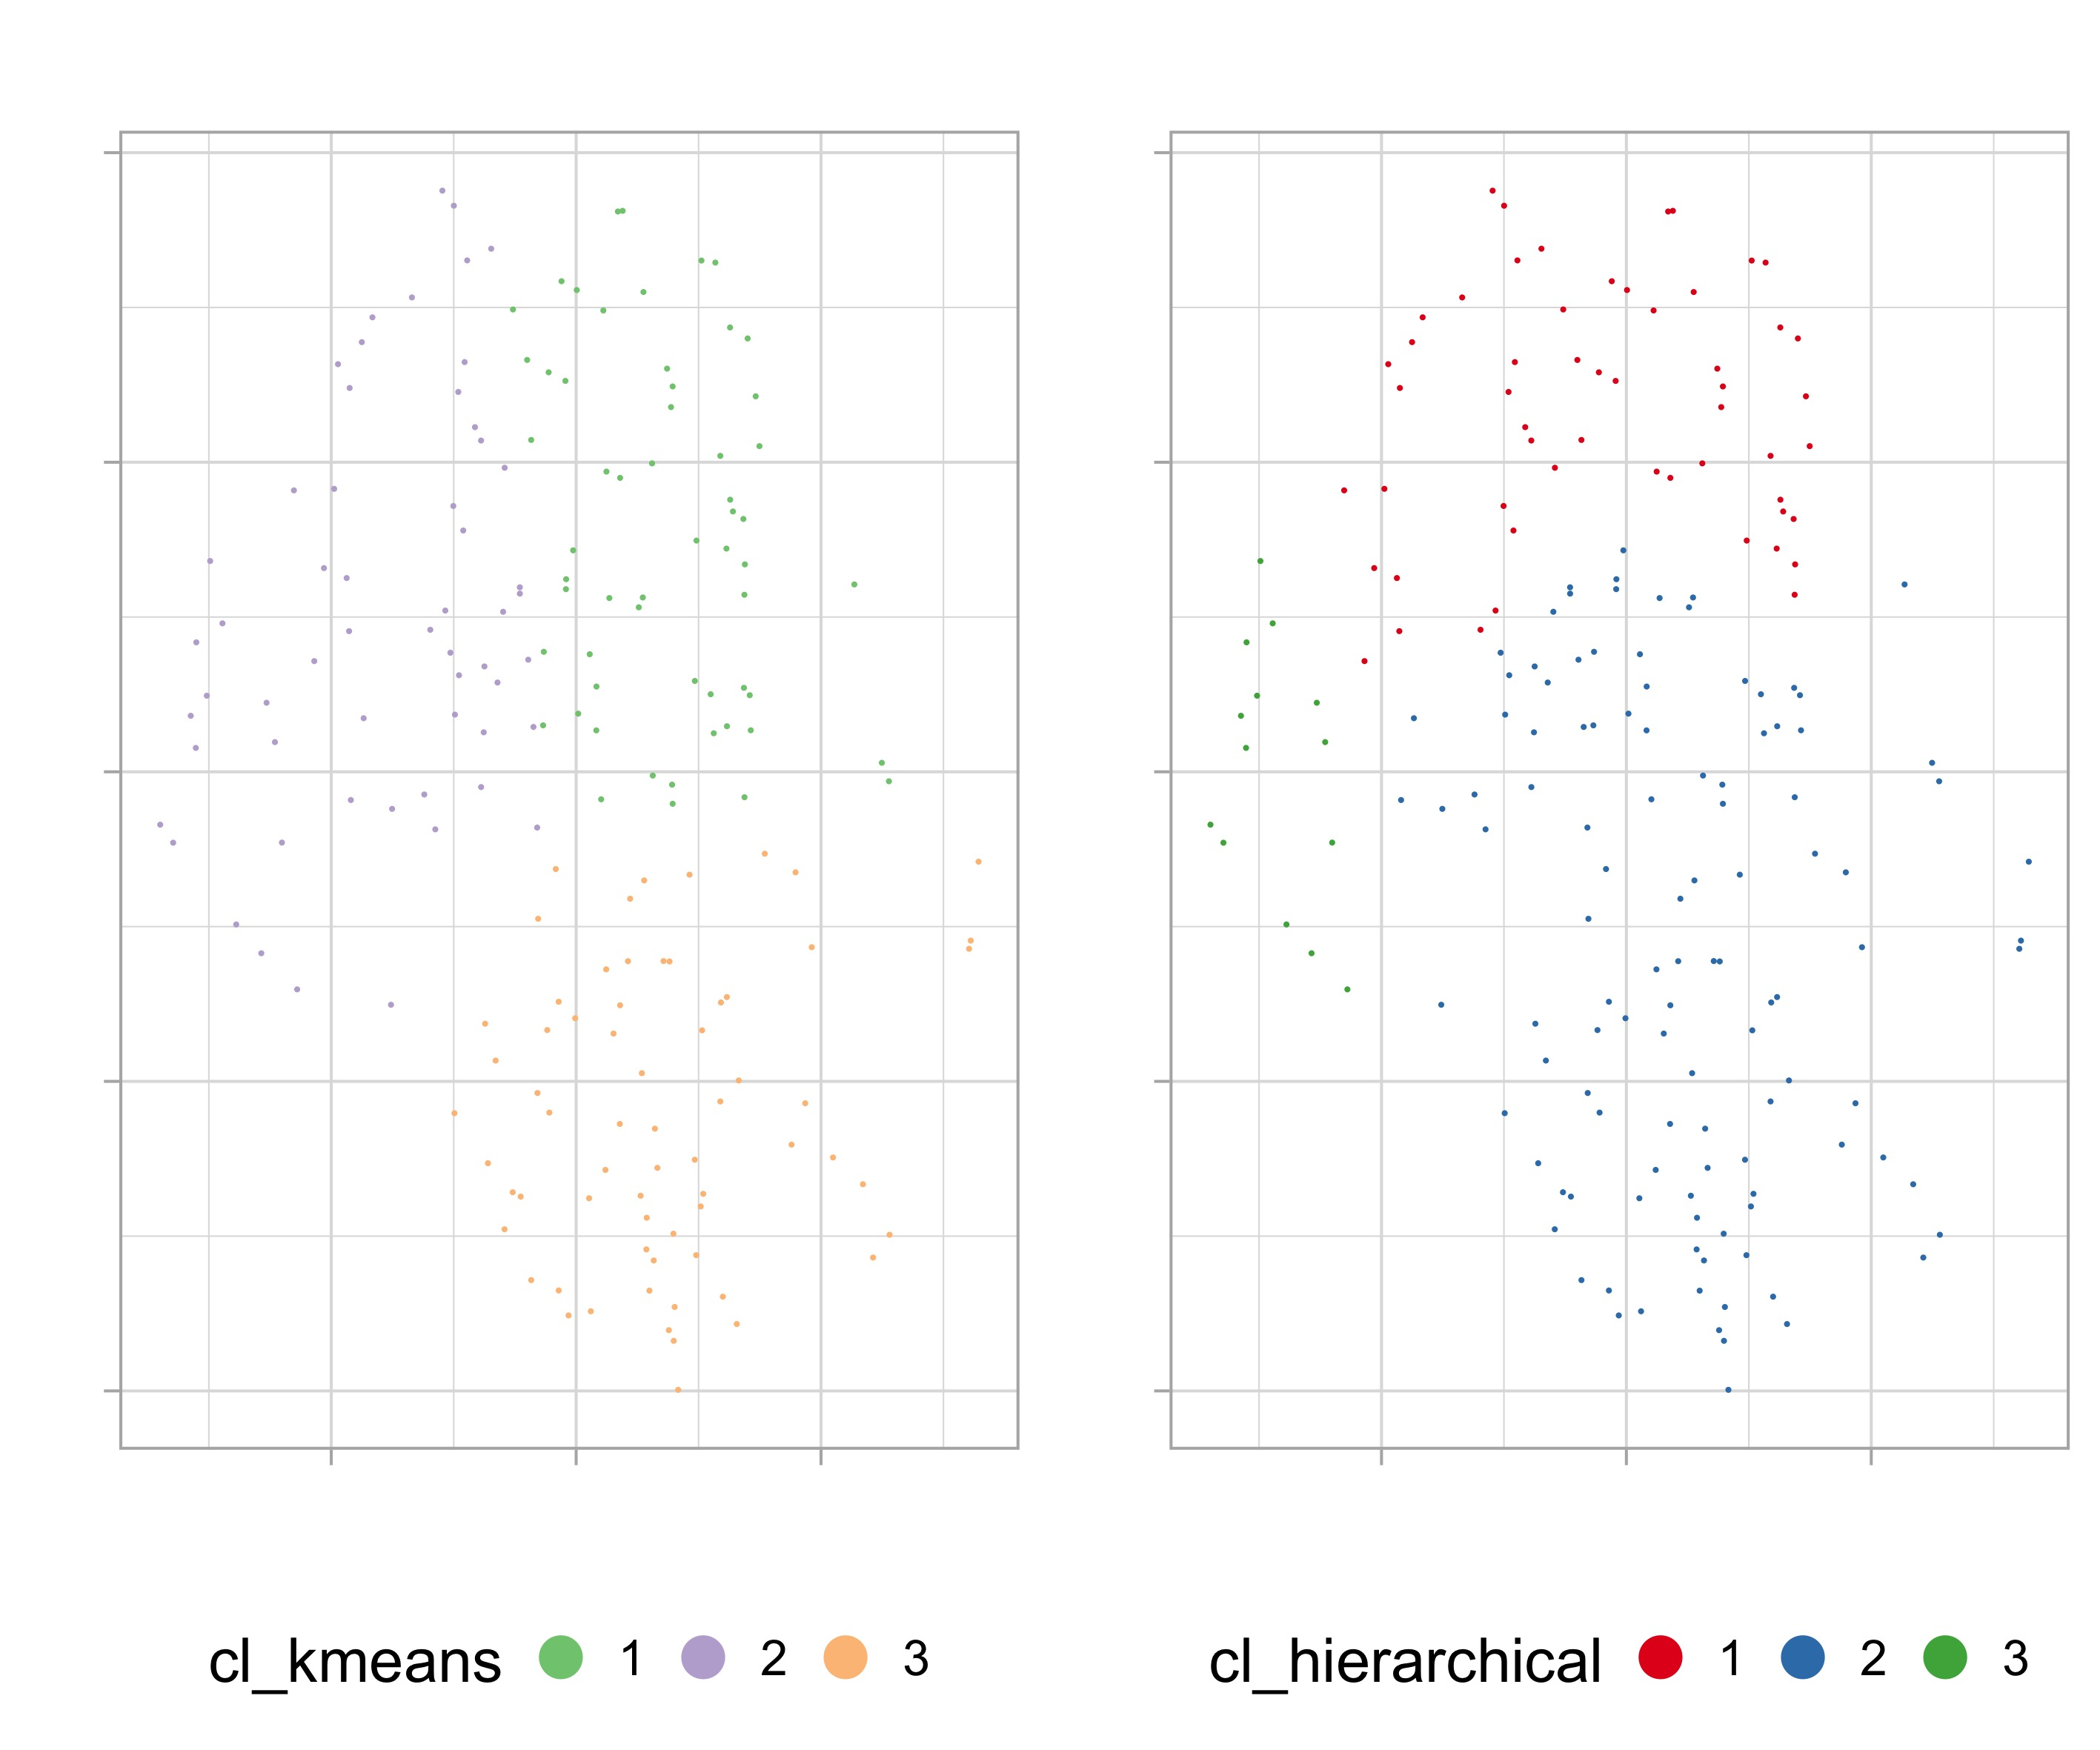
\includegraphics[width = 0.9\linewidth, height = 5cm]{Image/cluster.jpg}
        \caption{clustering}
        \end{subfigure}
        
    \end{figure}
    
    \item Principal component analysis
    
    \begin{figure}[H]
        
        \begin{subfigure}{0.5\textwidth}
        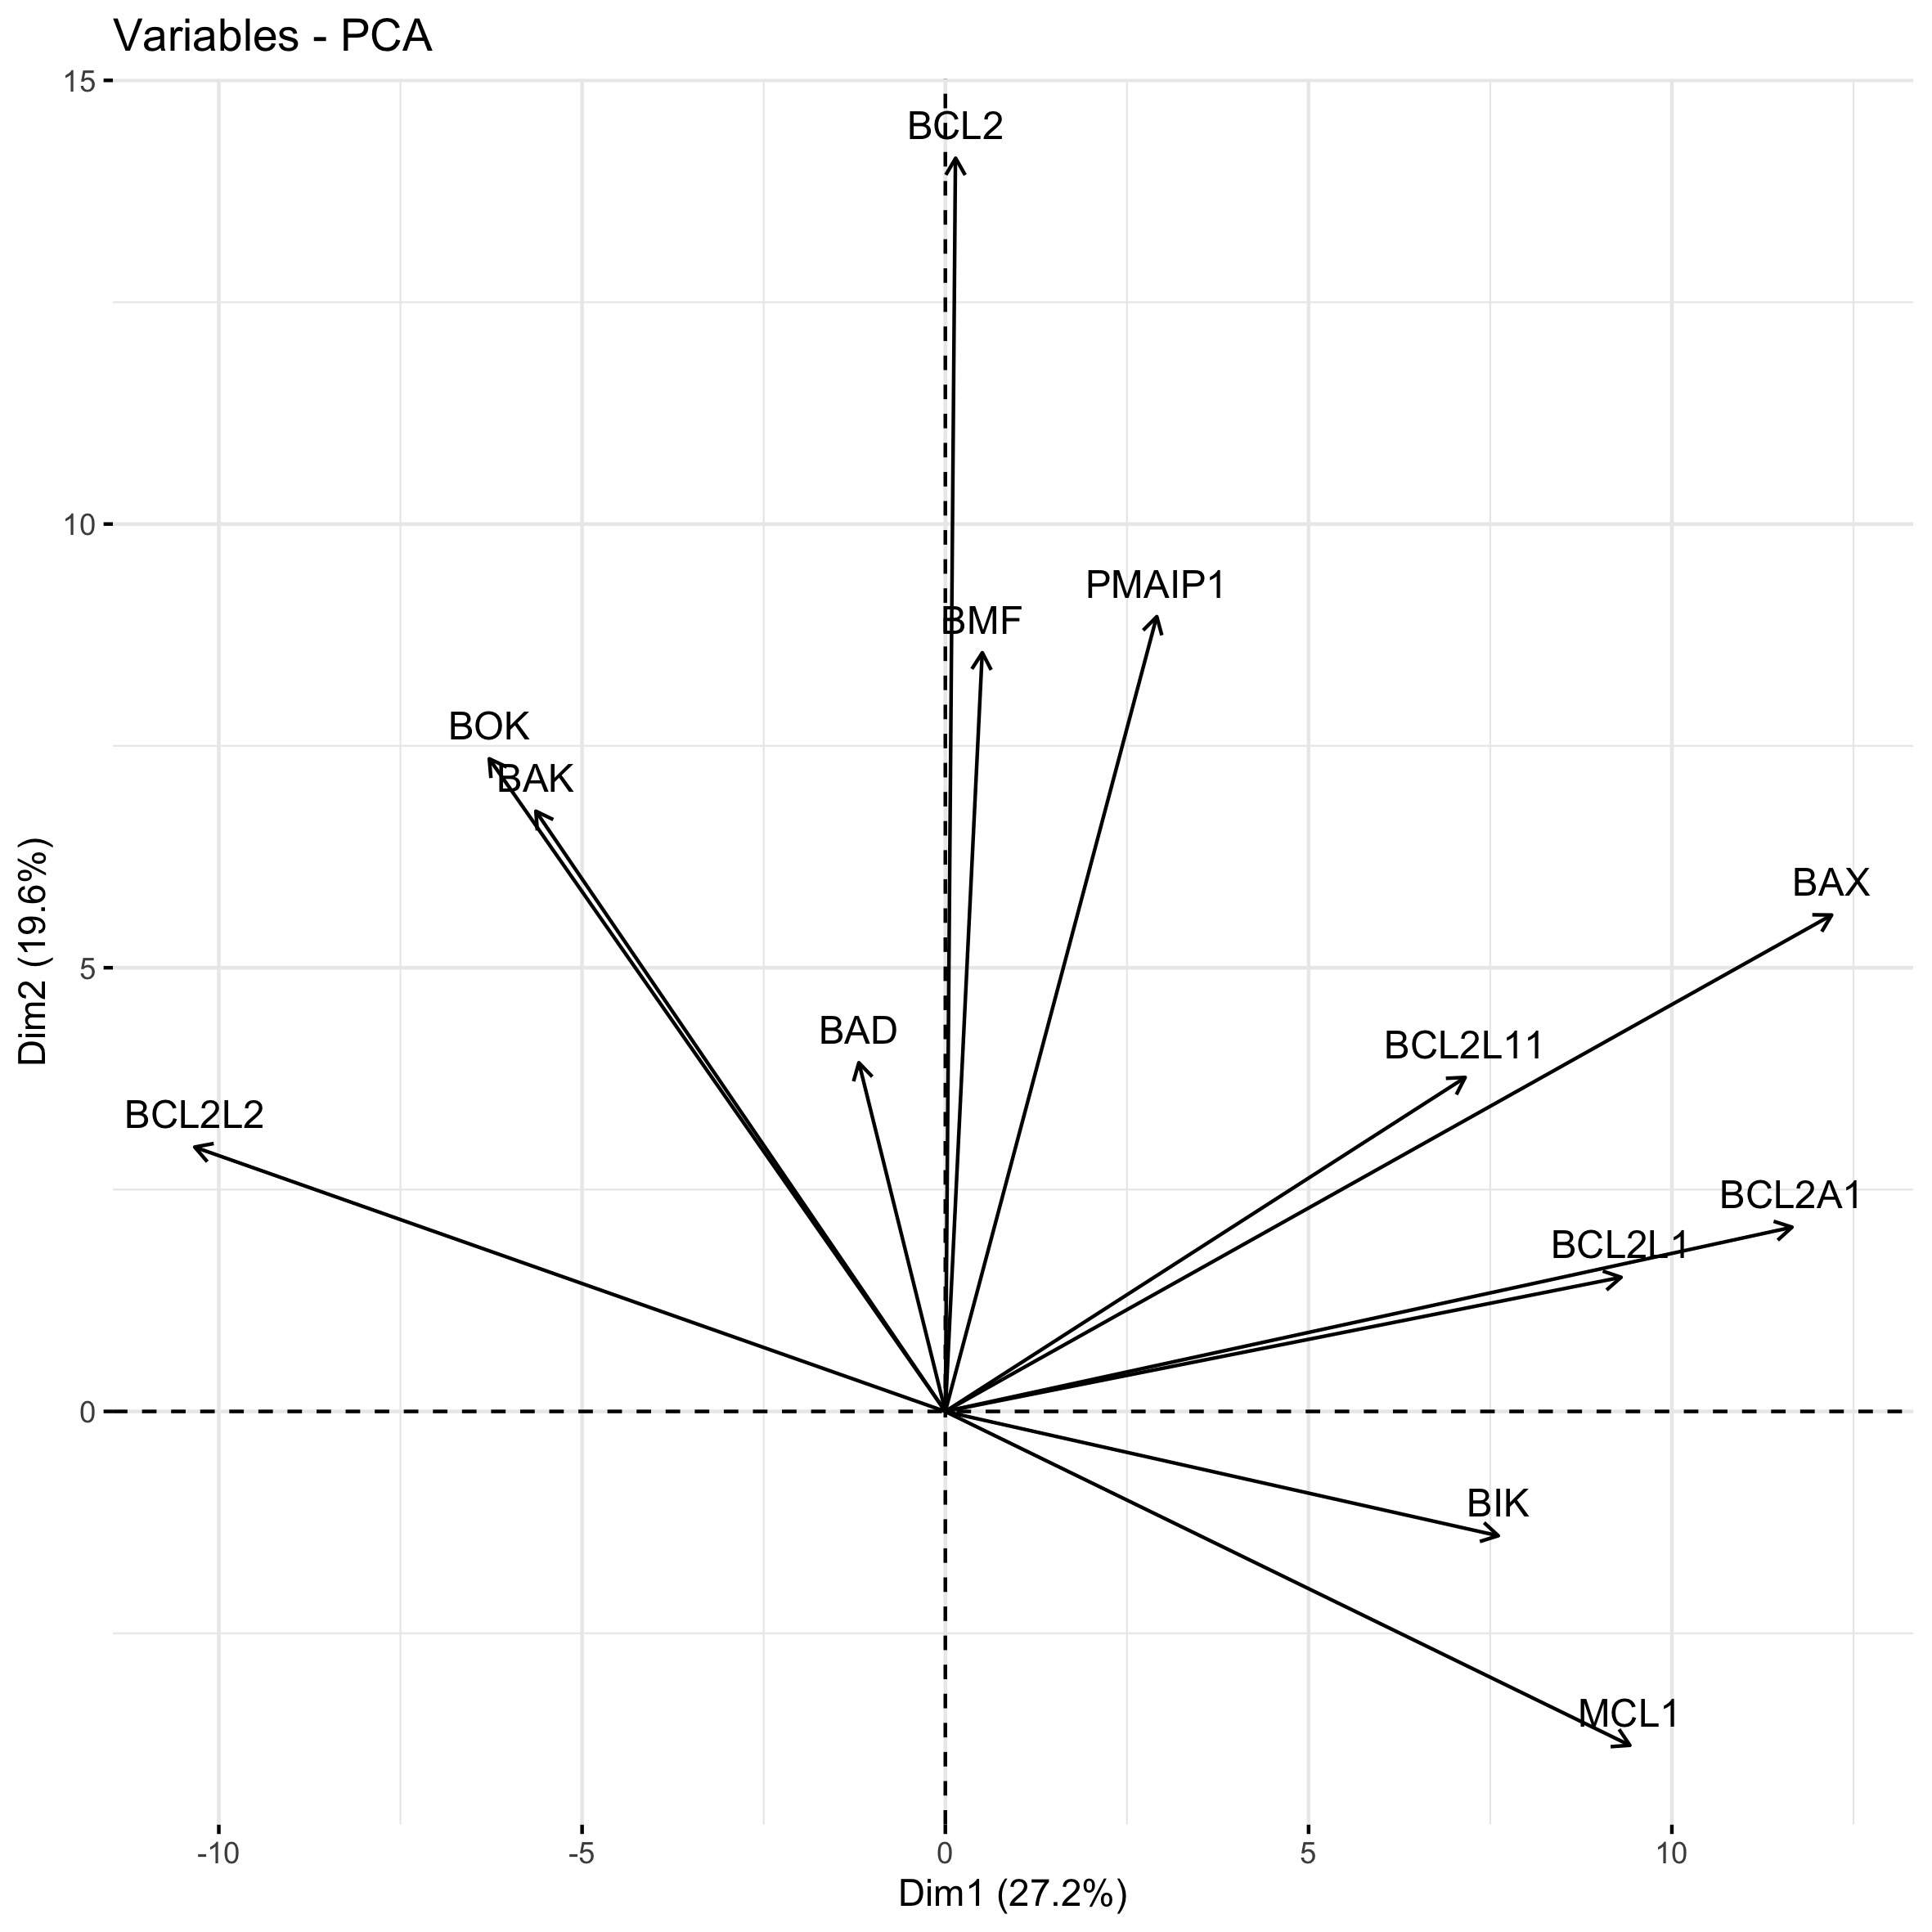
\includegraphics[width = 0.9\linewidth, height = 5cm]{Image/correlation_circle.jpg}
        \caption{Correlation circle}
        \end{subfigure}
        \begin{subfigure}{0.5\textwidth}
        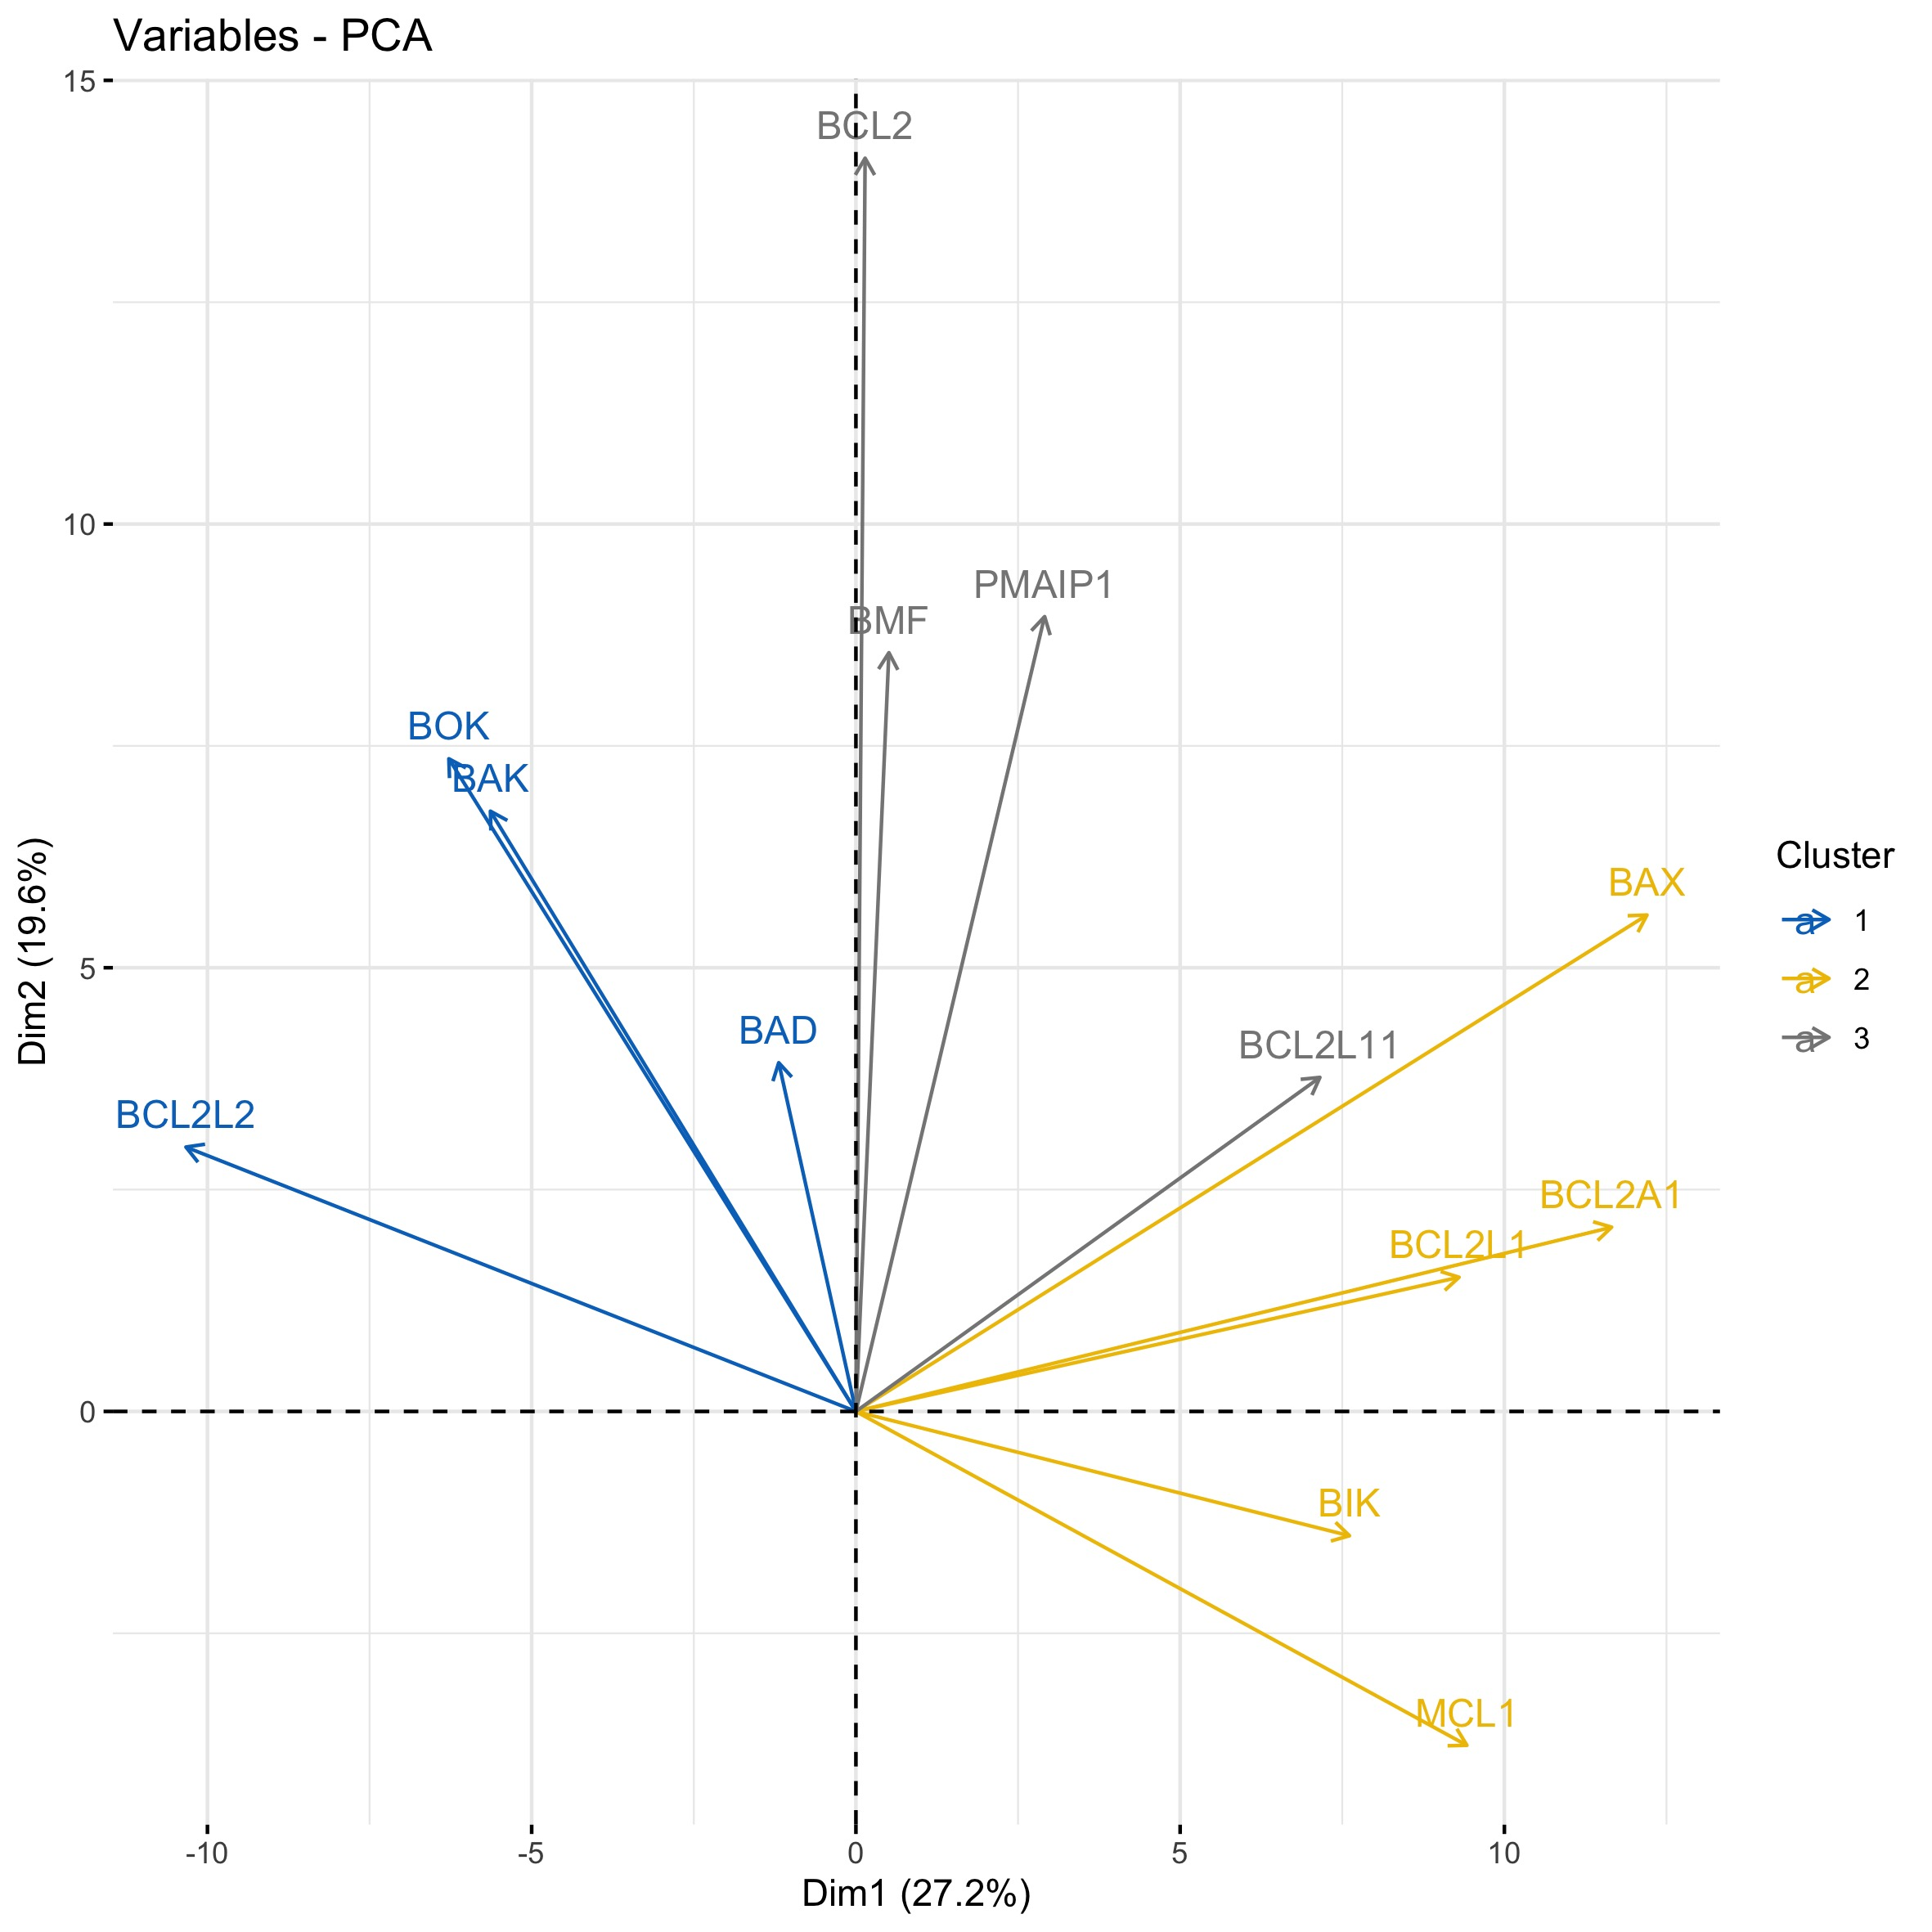
\includegraphics[width = 0.9\linewidth, height = 5cm]{Image/PCA_plot_grp.jpg}
        \caption{PCA with k-means clustering}
        \end{subfigure}
        
    \end{figure}
    
\end{enumerate}

\section*{Topic 3 BCL2 family expressions according to the groups}

\begin{enumerate}
    \item BCL2 super-expressor
    
    \begin{figure}[H]
        \begin{subfigure}{0.5\textwidth}
        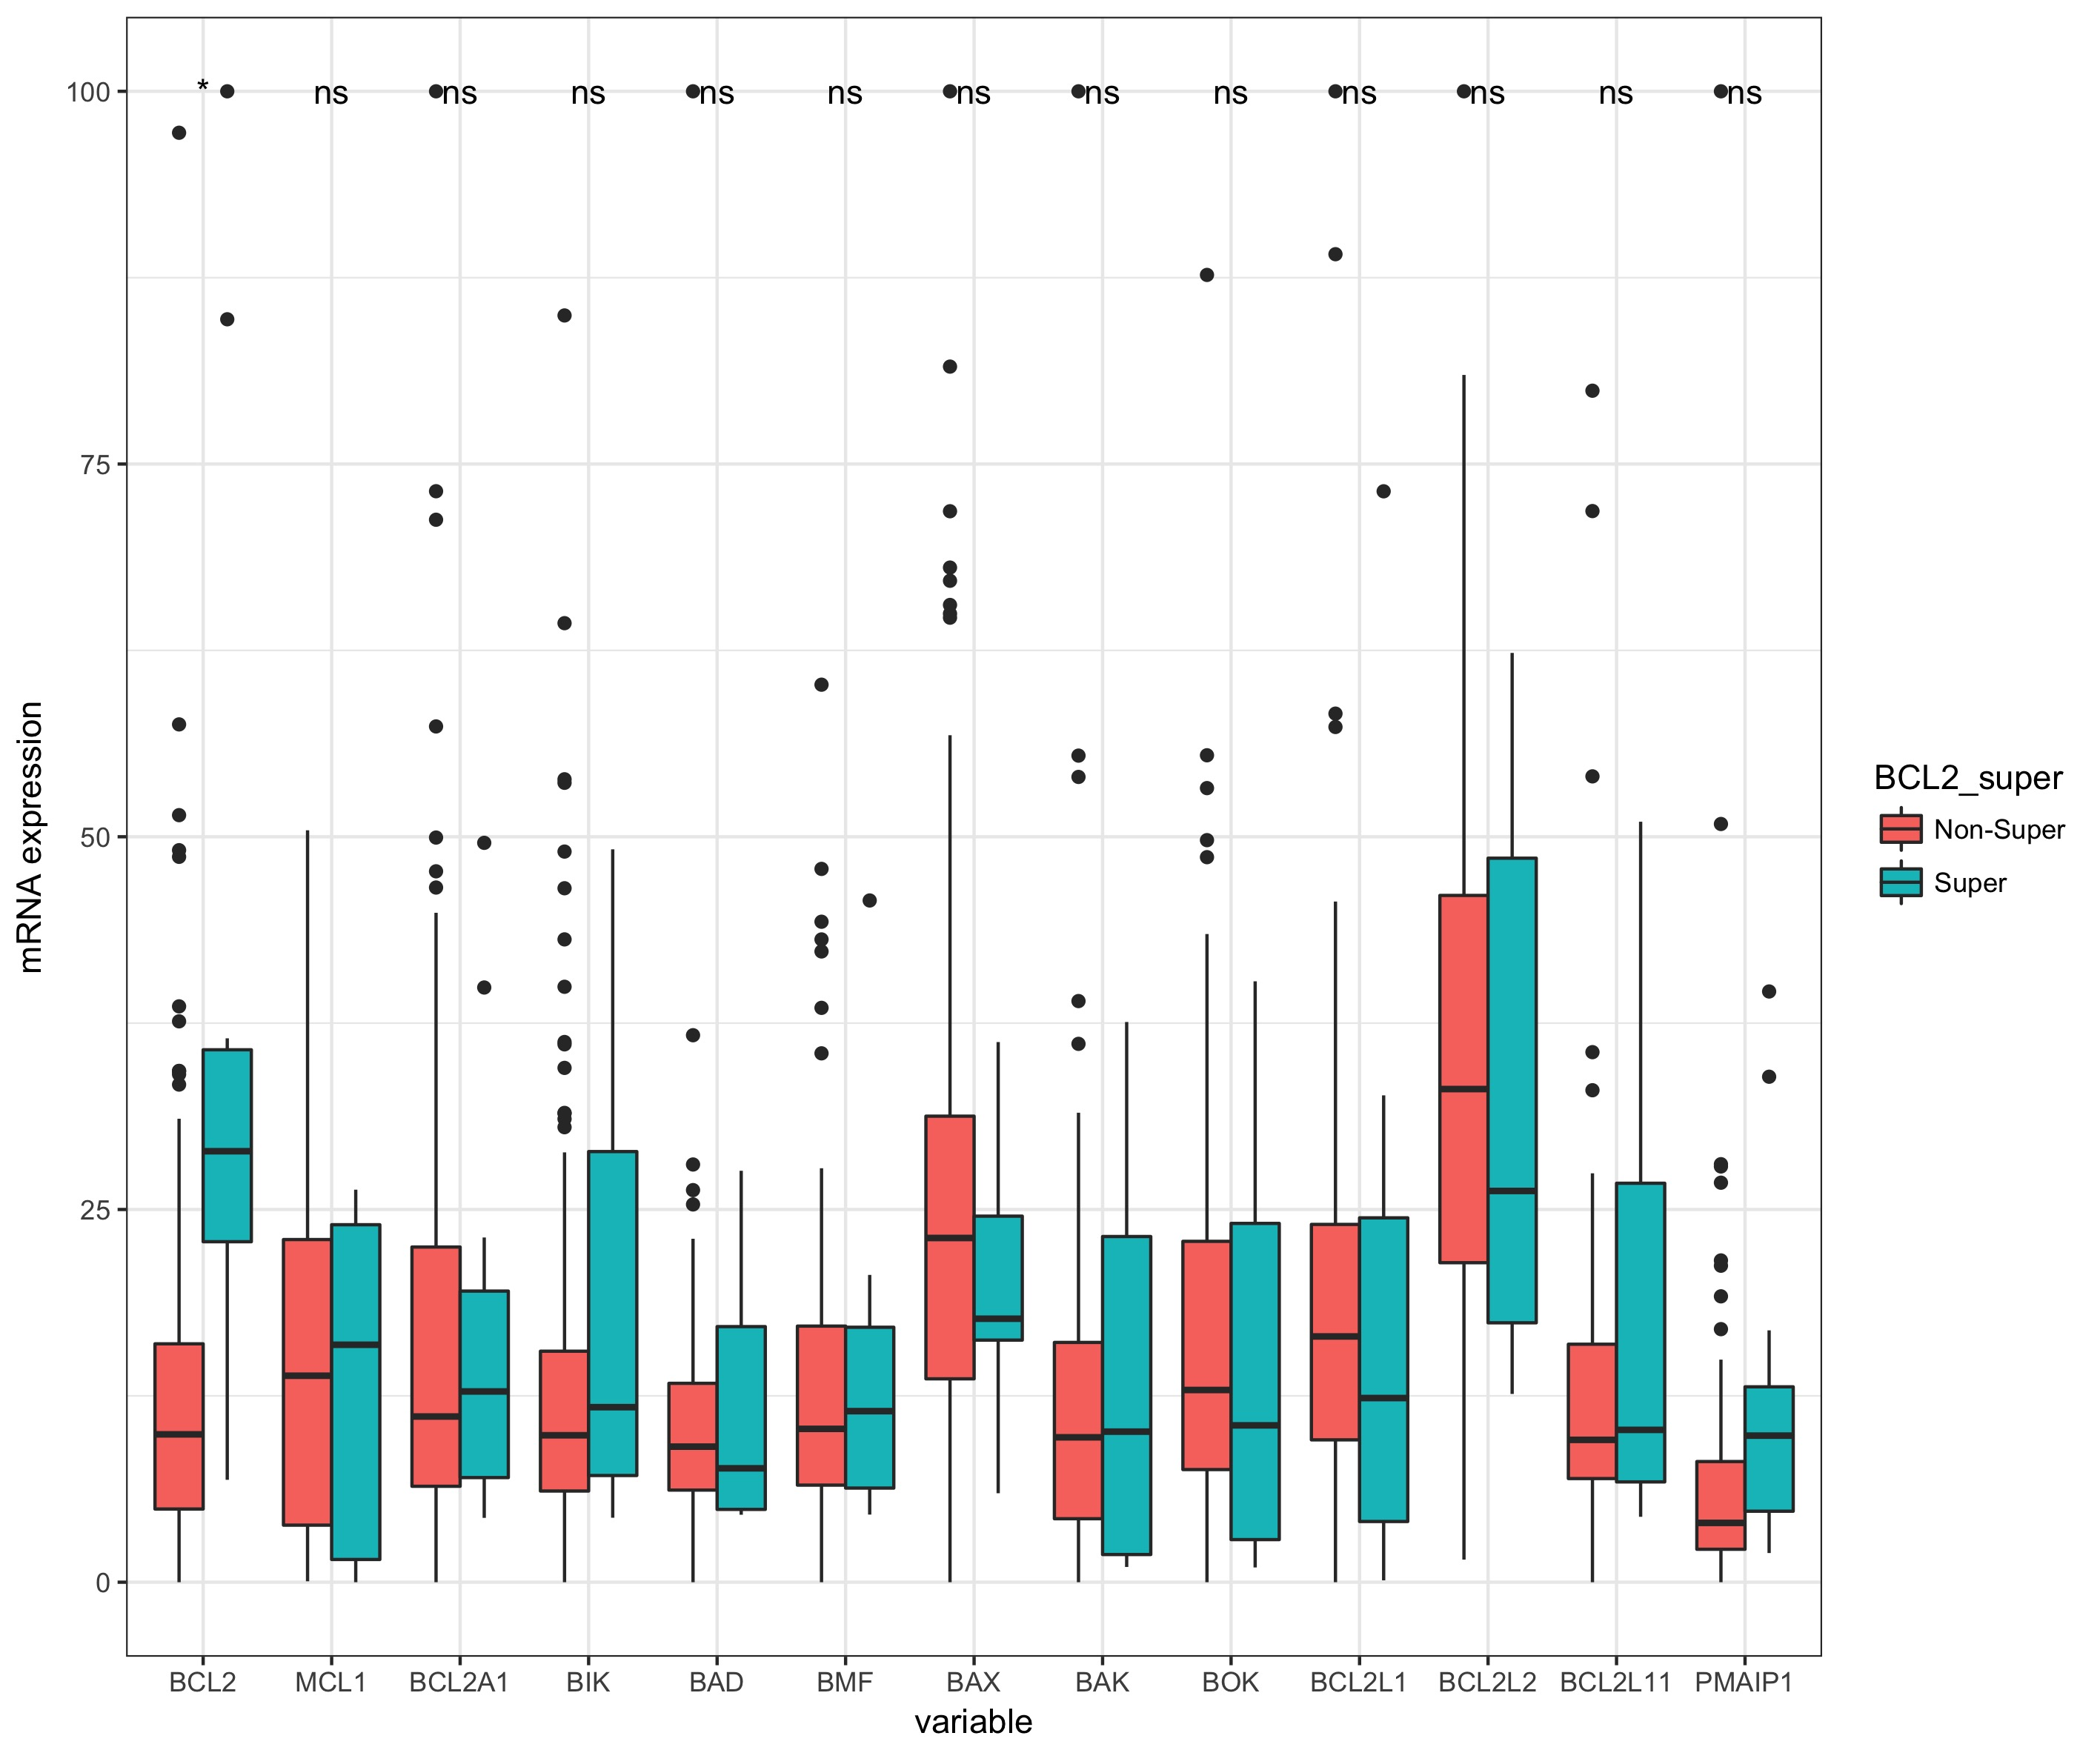
\includegraphics[width = 0.9\linewidth, height = 5cm]{Image/BCL2_Super_group.jpg}
        \caption{Compare mRNA expression by using the bar polots}
        \end{subfigure}
        \begin{subfigure}{0.5\textwidth}
        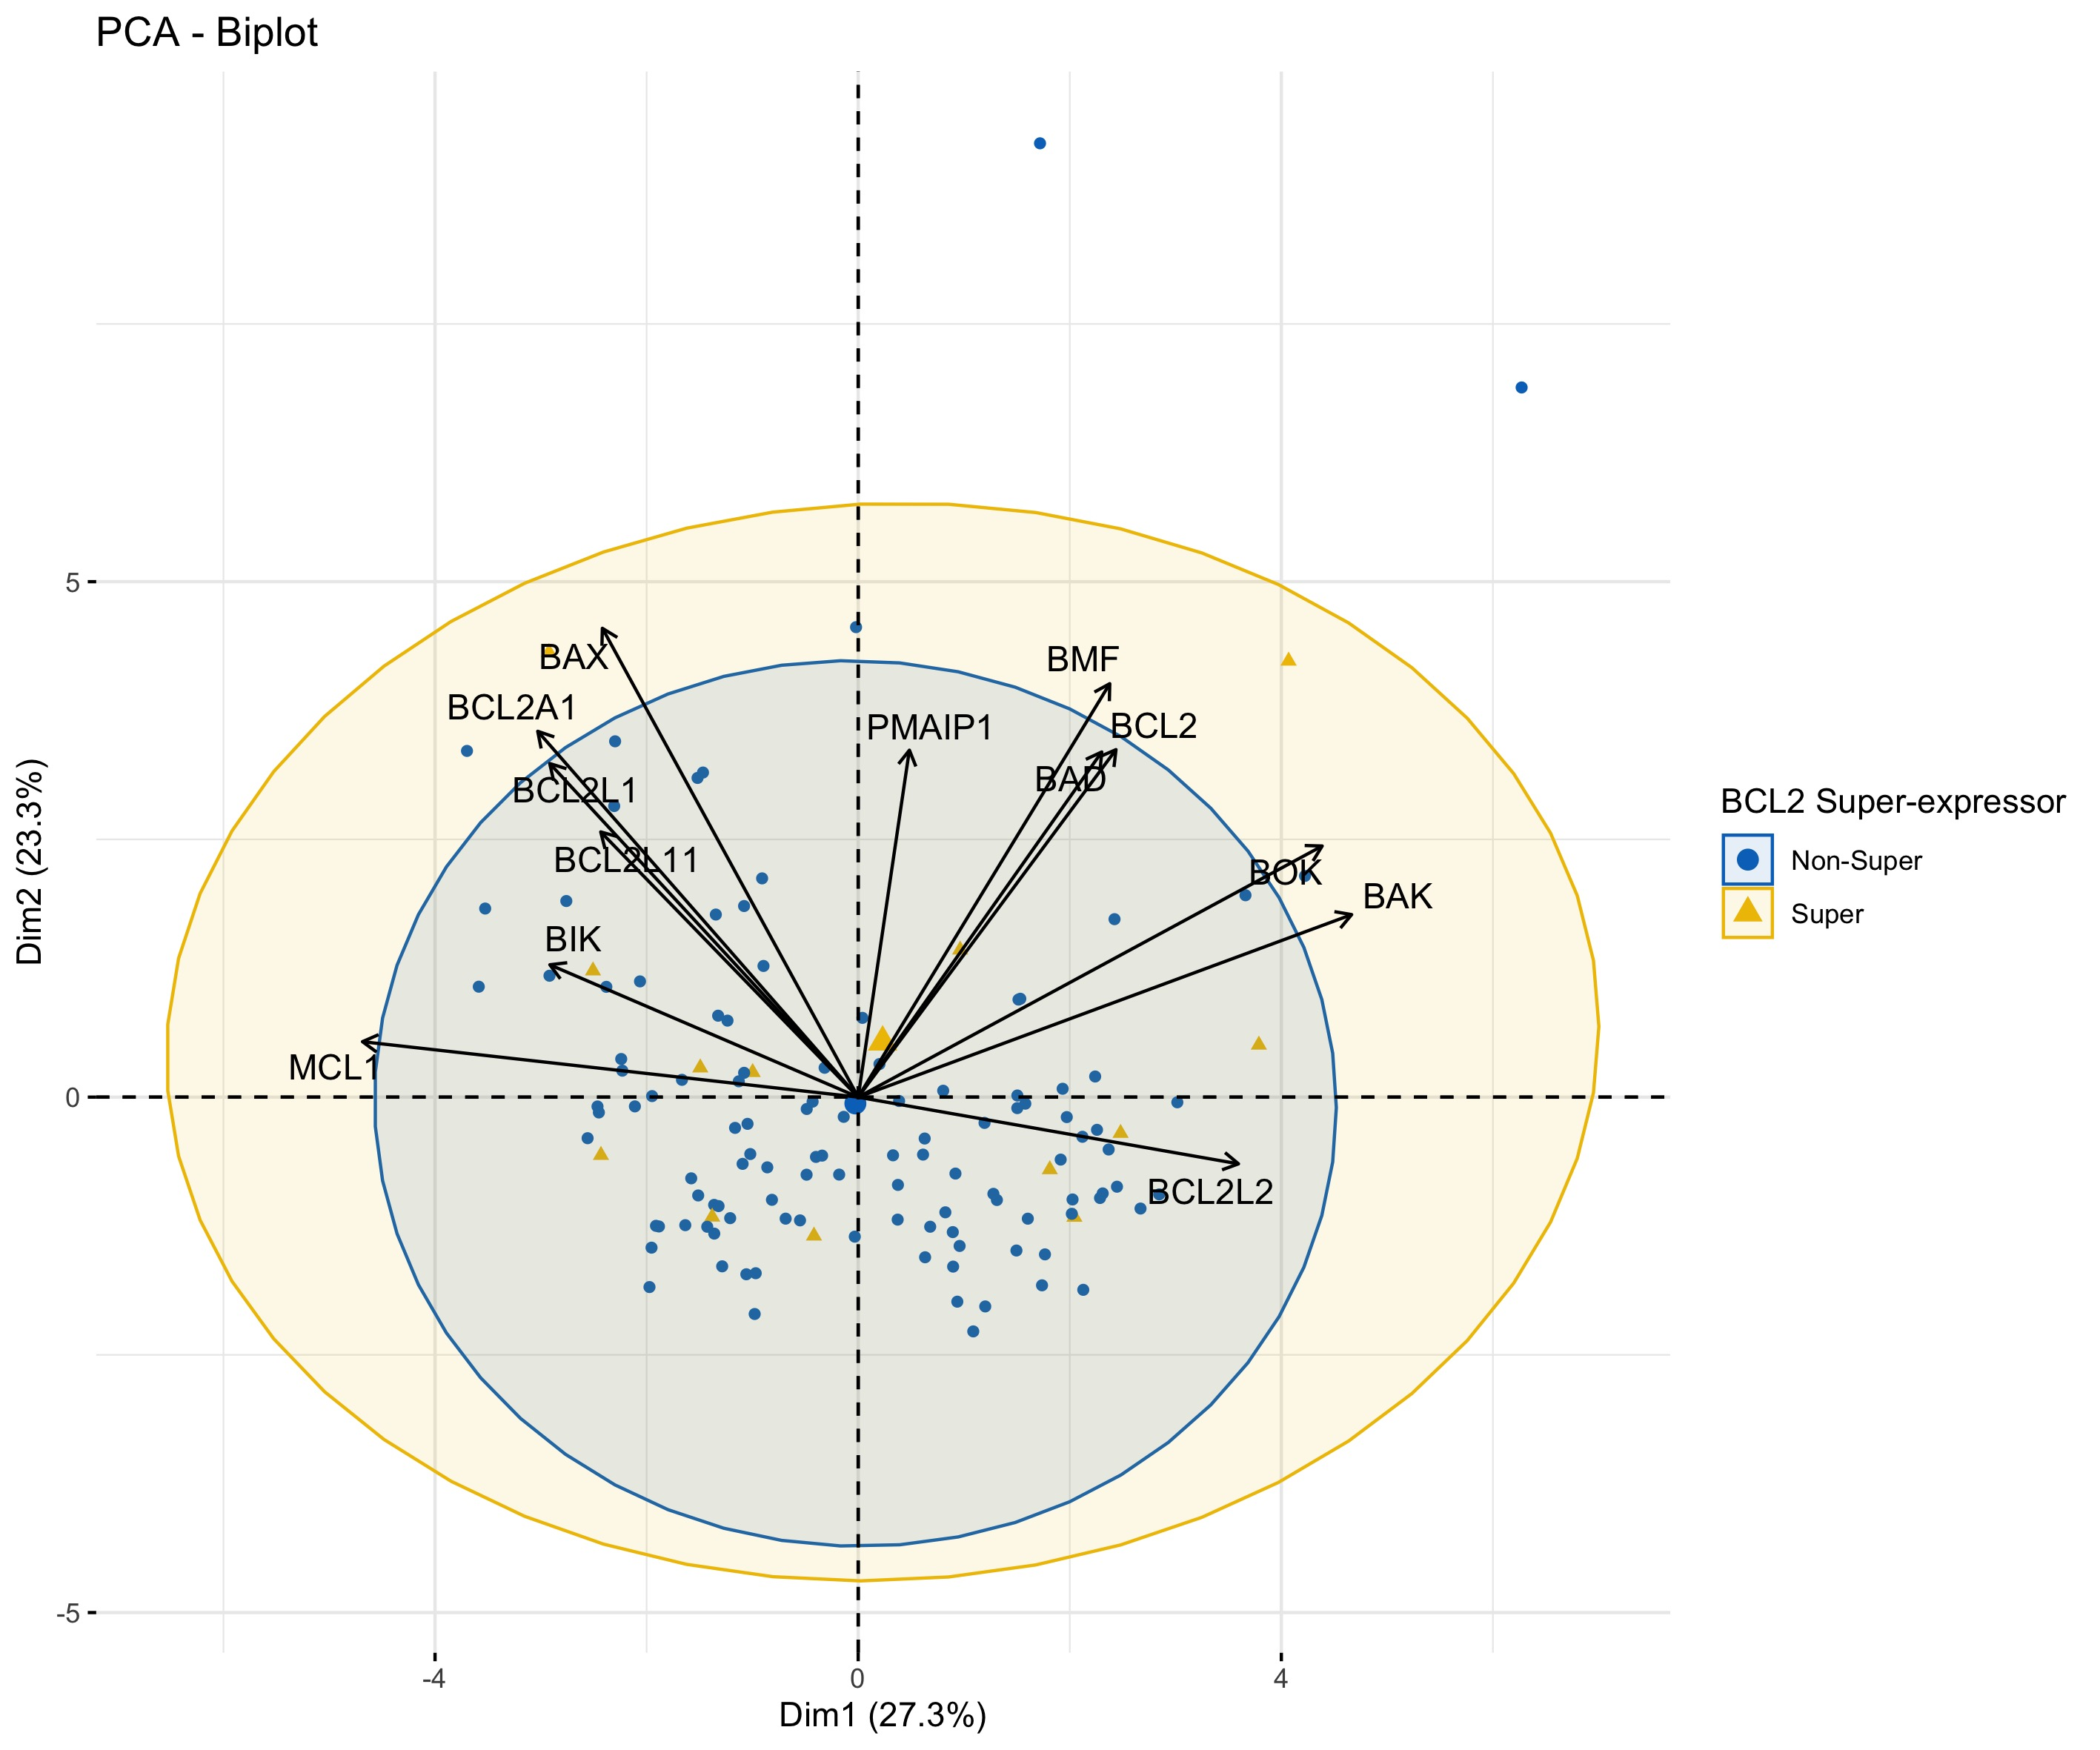
\includegraphics[width = 0.9\linewidth, height = 5cm]{Image/Super_PCA_biplot.jpg}
        \caption{PCA biplot according to the BCL2 super expressor}
        \end{subfigure}
    \end{figure}
    
    Besides BCL2, there is no significant difference between super-expressor and non-super-expressor.\\
    
    \item Cell Of Origin by nanostring
    
    \begin{figure}[H]
    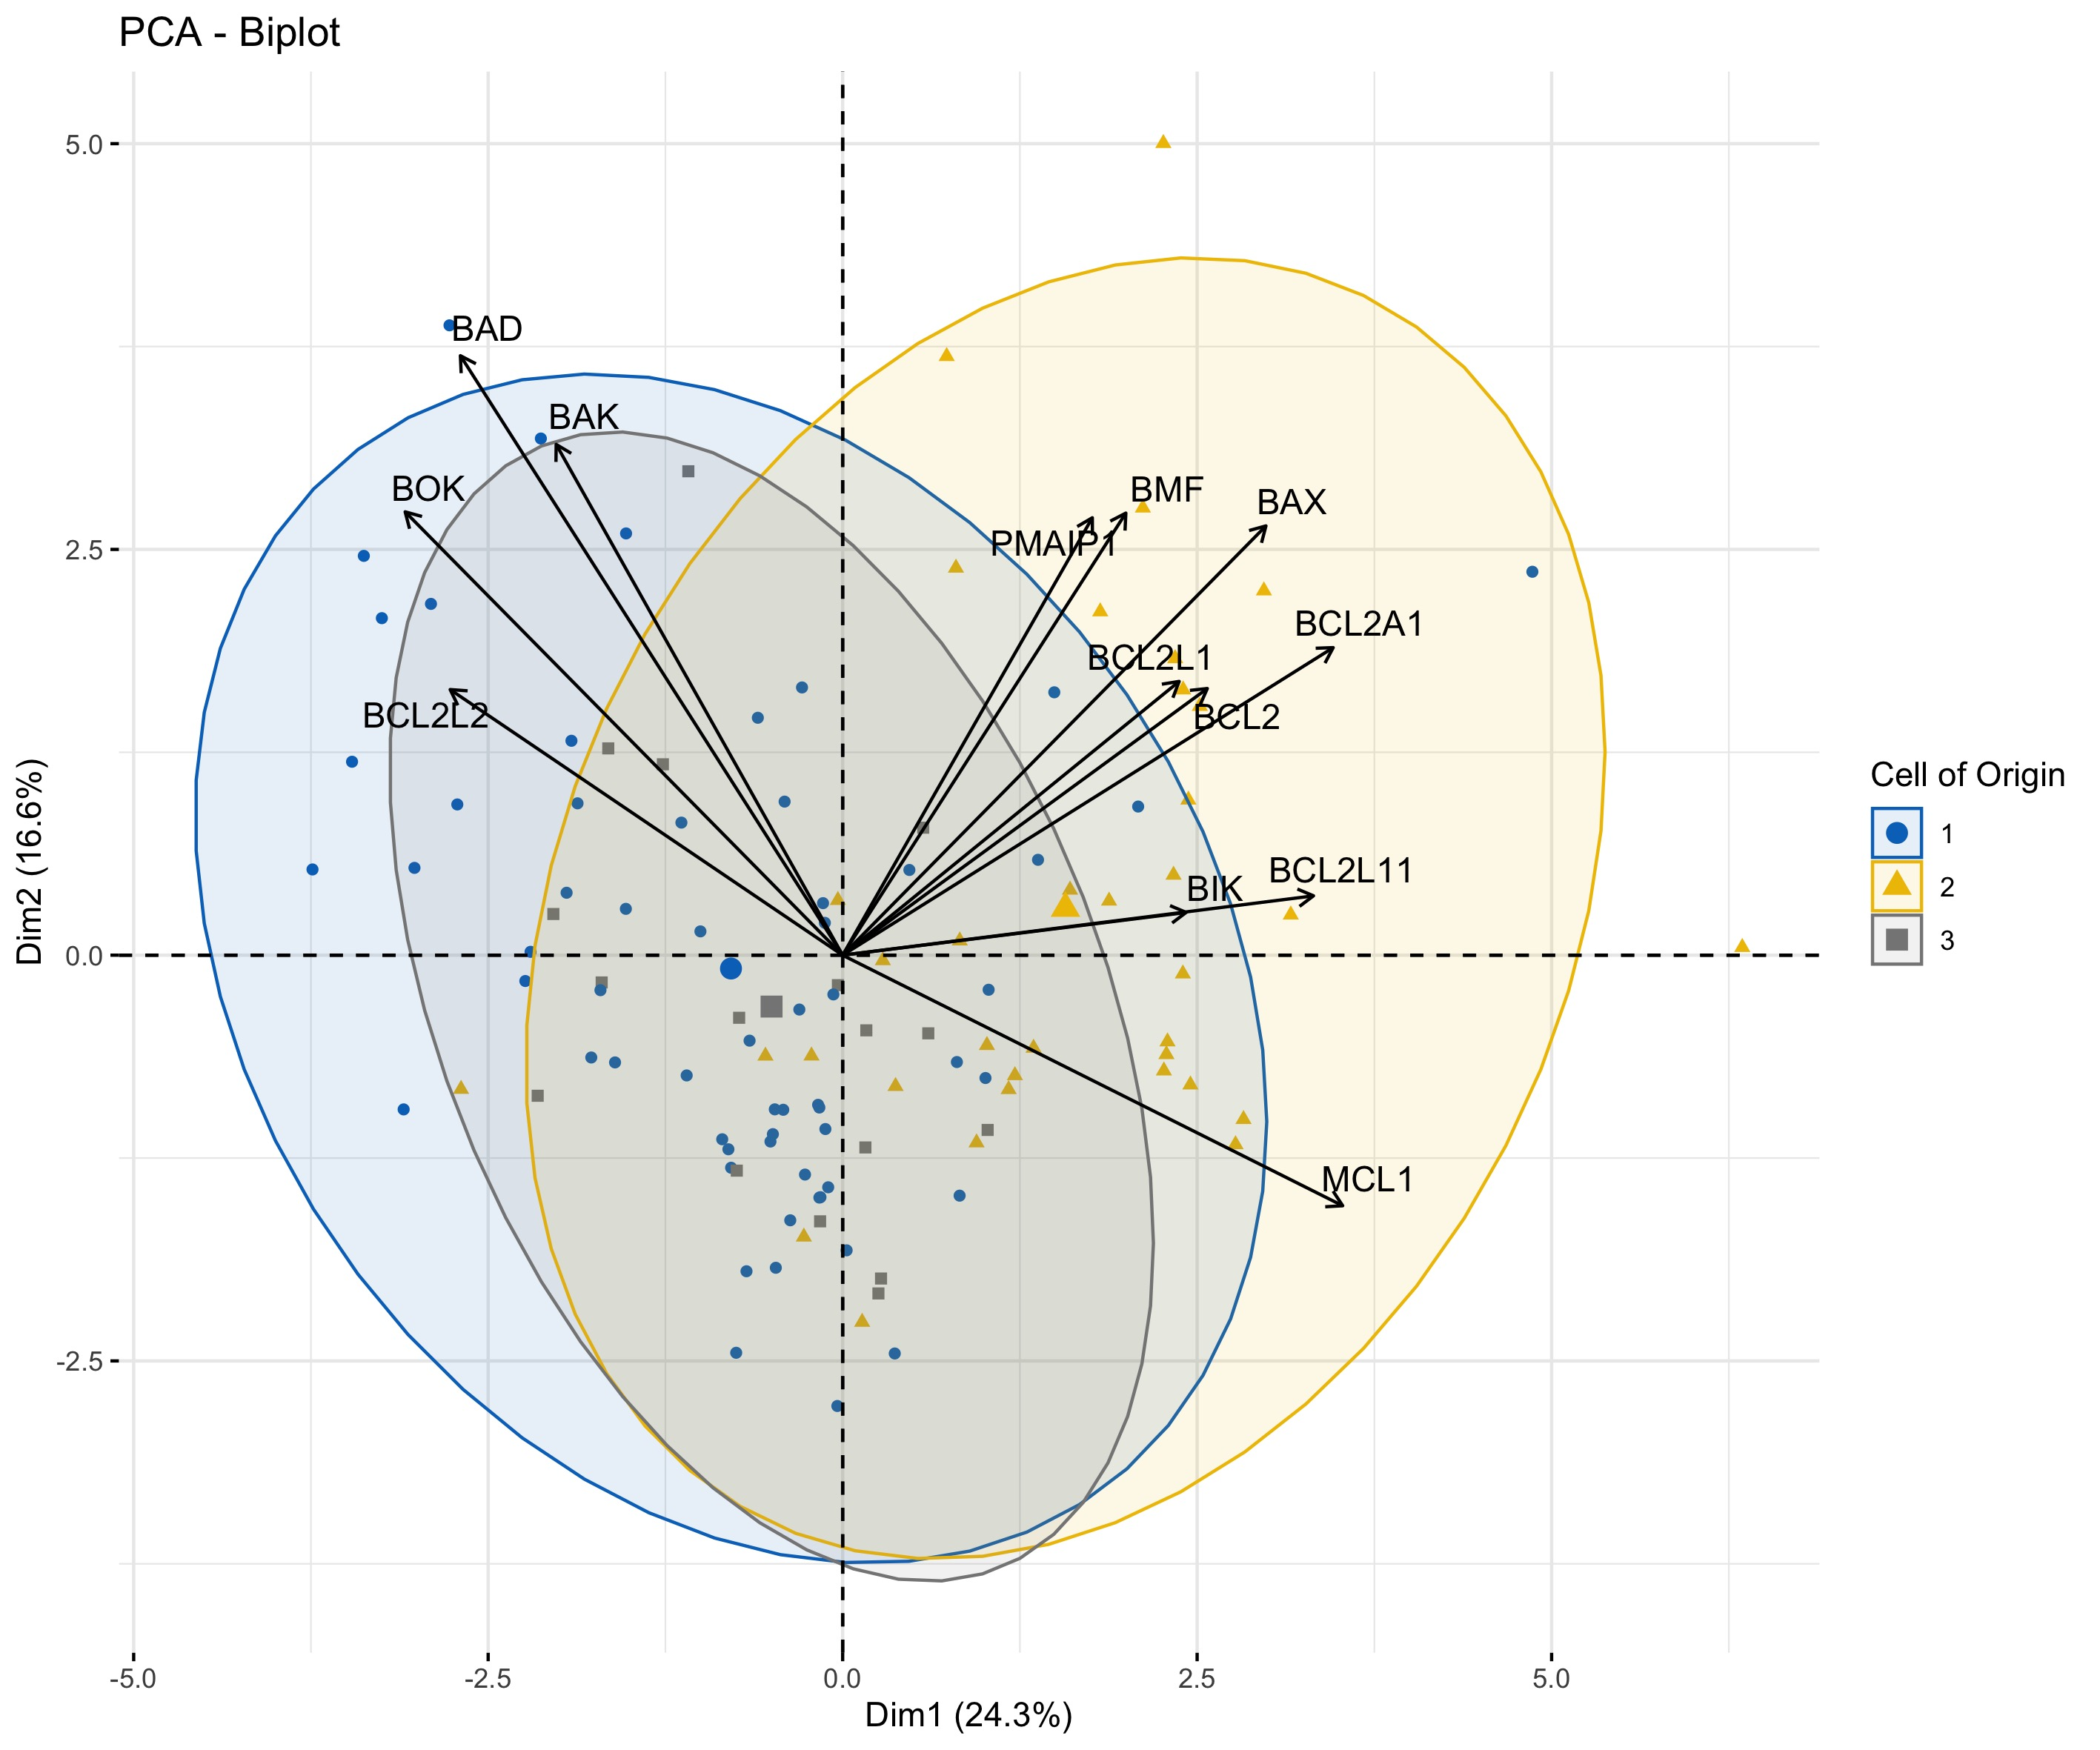
\includegraphics[width = 0.8\linewidth]{Image/COO_PCA_biplot.jpg}
    \caption{1: GCB, 2: ABC, 3: Unclassifiable}
    \end{figure}
    
    In GCB subgroup, BAX, BAD, BOK, BCL2L2 are characteristically more expressed than ABC subgroup. And most of these proteins are included in the pro-apoptotic effectors. Interestingly, GCB subgroup and unclassifiable subgroup showed similar expression pattern.\\
    In ABC subgroup, BAX, BMF, PMAIP1, BCL2, BCL2L1, BCL2L11, BIK, MCL1 are more expressed than GCB subgroup. 
    
    \item Cell Of Origin by Hans classification
    
    \begin{figure}[H]
        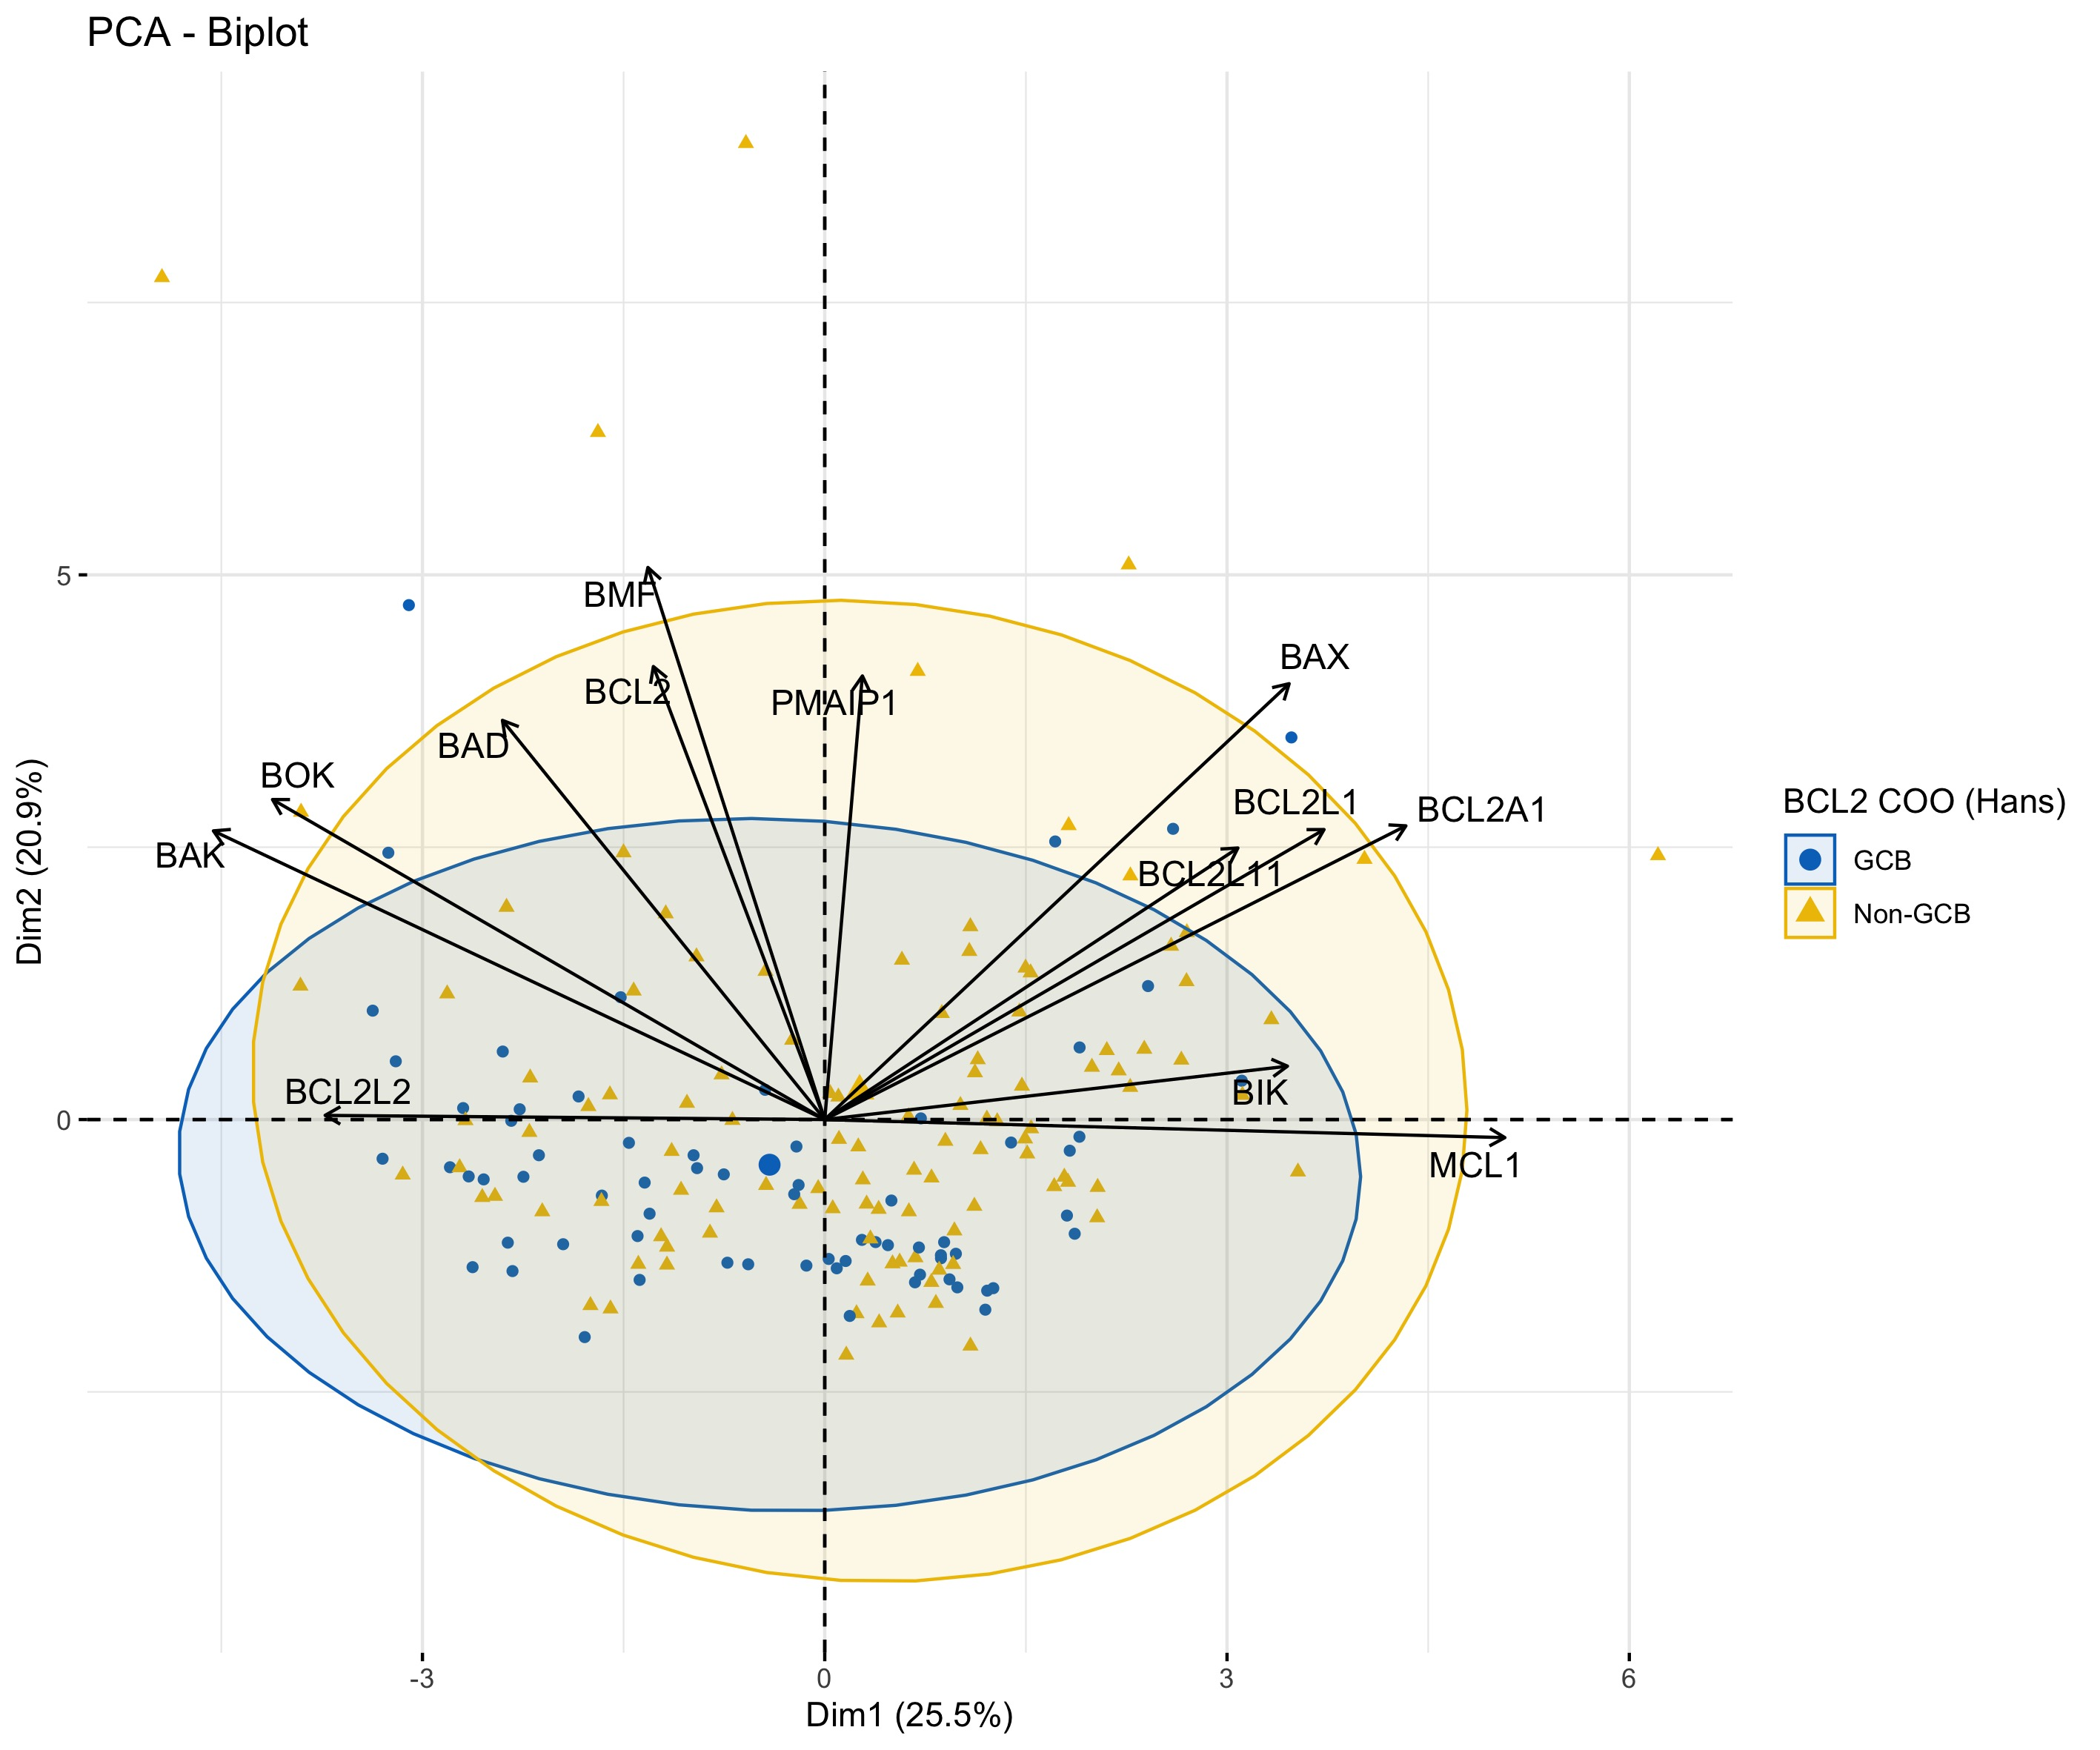
\includegraphics[width = 0.8\linewidth]{Image/COO_Hans_biplot.jpg}
        \caption{PCA biplot according to the COO by Hans classification}
    \end{figure}
    
    In COO subgroups classified by Hans classificaion, there is no identifiable tendency in BCL2 family expression.
    
    \item IPI groups
    
    \begin{figure}[H]
        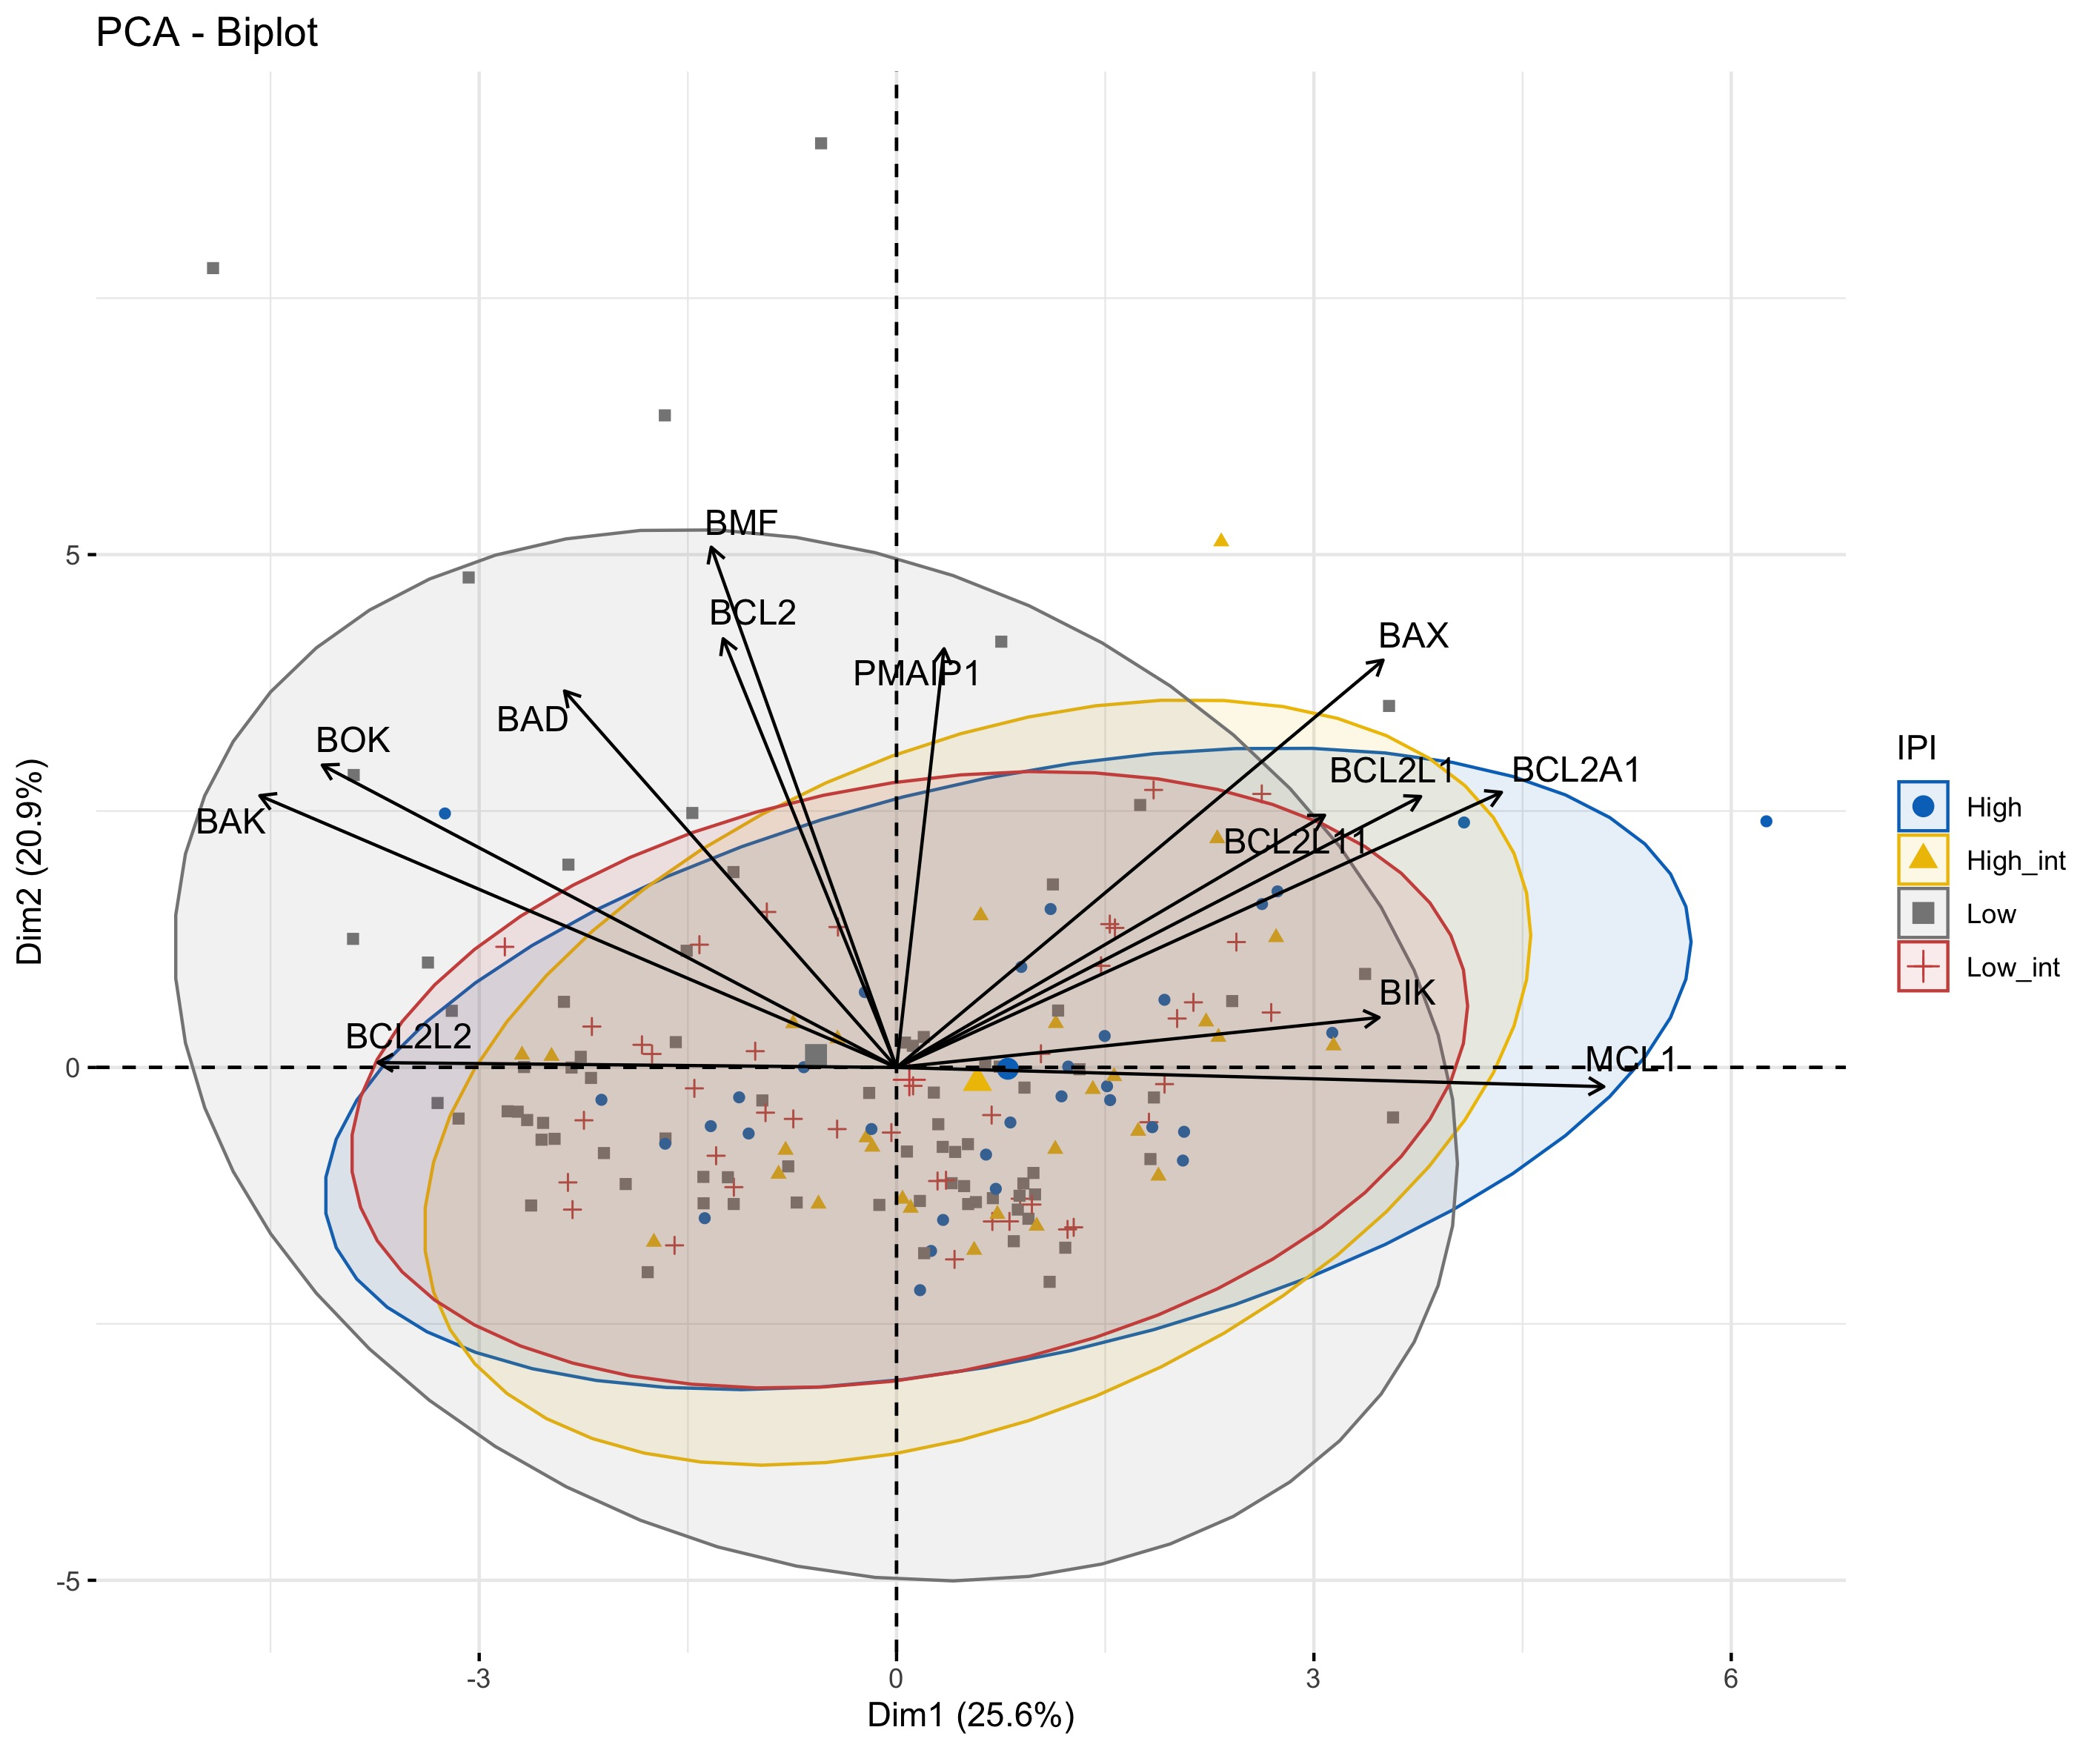
\includegraphics[width = 0.8\linewidth]{Image/IPI_biplot.jpg}
        \caption{PCA biplot according to the IPI groups}
    \end{figure}
    
    Interestingly, pro-apoptotic family members are more expressed in low IPI group (IPI 0-1). Although high BCL2 expression is associated with poor prognosis, it shows high value in low IPI group.
    
\end{enumerate}

\end{document}
